\documentclass[svgnames]{beamer}[10]
% \usepackage{babel}
\usepackage{beamerthemesplit}
\usepackage{epsfig}
\usepackage{subfigure}
\usepackage{url}
\usepackage{srcltx}
\usepackage{hyperref}
\usepackage{soul}
\usepackage{natbib}
\usepackage{apalike}
\usepackage{graphicx}
\usepackage{booktabs} % Top and bottom rules for table
\usepackage[font=small,labelfont=bf]{caption} % Required for specifying captions to tables and figures
\usepackage{wrapfig} % Allows wrapping text around tables and figures
\usepackage{lipsum}
\usepackage{adjustbox}
\usepackage[absolute,overlay]{textpos}
\usepackage{lmodern}
\usepackage{amsmath}
\usepackage{amsfonts}
\usepackage{color}
\usepackage{array}
\usepackage{multirow}
\usepackage{multicol}
\usepackage{rotating}
\usepackage{pgf}
\usepackage{pgfpages}
\usepackage{pgfplots}
\usepackage{pgfplotstable}
\usepackage{tikz}
\usepackage{tikz-qtree}
\usepackage{tikz-dependency}

\graphicspath{{figures/}} % Location of the graphics files

\definecolor{lightblue}{rgb}{.90,.95,1}
\sethlcolor{lightblue}
\renewcommand<>{\hl}[1]{\only#2{\beameroriginal{\hl}}{#1}}
\definecolor{kugreen}{RGB}{50,93,61}
\definecolor{kugreenlys}{RGB}{132,158,139}
\definecolor{kugreenlyslys}{RGB}{173,190,177}
\definecolor{kugreenlyslyslys}{RGB}{214,223,216}
\definecolor{ku}{RGB}{144,26,30}
\definecolor{ku-yellow}{RGB}{255,249,25}
\setbeamercovered{transparent}
\mode<presentation>
\usetheme[numbers,compress,sidebarshades]{PaloAlto}
\setbeamertemplate{footline}[frame number]

\usetikzlibrary{trees,arrows.meta,graphs,graphs.standard,graphdrawing,quotes,shapes}
\usegdlibrary{layered,trees}
\pgfplotsset{compat=1.17}
\setbeamertemplate{sidebar left}{}
\tikzset{
  invisible/.style={opacity=0},
  visible on/.style={alt={#1{}{invisible}}},
  alt/.code args={<#1>#2#3}{%
    \alt<#1>{\pgfkeysalso{#2}}{\pgfkeysalso{#3}} % \pgfkeysalso doesn't change the path
  },
}
\captionsetup{labelformat=empty}

\makeatletter
\pgfdeclareshape{vector}{
	  \inheritsavedanchors[from={rectangle}]
	  \inheritbackgroundpath[from={rectangle}]
	  \inheritanchorborder[from={rectangle}]
	  \foreach \x in {center,north east,north west,north,south,south east,south west,east,west}{
	    \inheritanchor[from={rectangle}]{\x}
	  }

    \backgroundpath{
      \pgftransformshift{\pgfpoint{-16pt}{-4pt}}
		  \draw[rounded corners=2pt] (0,0) rectangle (32pt,8pt);
    }

    \beforebackgroundpath{
      \draw[step=8pt,help lines,-] (8pt,.1pt) grid (24pt,7.9pt);
    }
}
\makeatother

  \usecolortheme[named=kugreen]{structure}
  \useinnertheme{circles}
  \usefonttheme[onlymath]{serif}
  \setbeamercovered{transparent}
  \setbeamertemplate{blocks}[rounded][shadow=true]
  
\makeatletter
\newcommand\SoulColor{%
  \let\set@color\beamerorig@set@color
  \let\reset@color\beamerorig@reset@color}
\makeatother
\SoulColor

% Outline slides
\AtBeginSection[]
{\begin{frame} \frametitle{Outline} \tableofcontents[currentsection,currentsubsection] \end{frame}}

\AtBeginSubsection[]
{\begin{frame} \frametitle{Outline} \tableofcontents[currentsection,currentsubsection] \end{frame}}

% \logo{\includegraphics[width=0.8cm]{KULogo}}
%\useoutertheme{infolines} 
\title{Universal Conceptual Cognitive Annotation}
\subtitle{Cross-lingual Semantic Representation for NLP with UCCA}
\author{
%   \textbf{Omri Abend},
%   \textbf{Dotan Dvir} \\
%   Hebrew University of Jerusalem \\
  \textbf{Daniel Hershcovich} \\
  University of Copenhagen \\
%   \textbf{Jakob Prange},
%   \textbf{Nathan Schneider} \\
%   Georgetown University
}
% \date{Tutorial at COLING 2020}
\date{Parsing, Evaluation and Applications}

\begin{document}
\frame{\titlepage}

% \section{Bird's Eye View}
% \begin{frame}{UCCA}
%     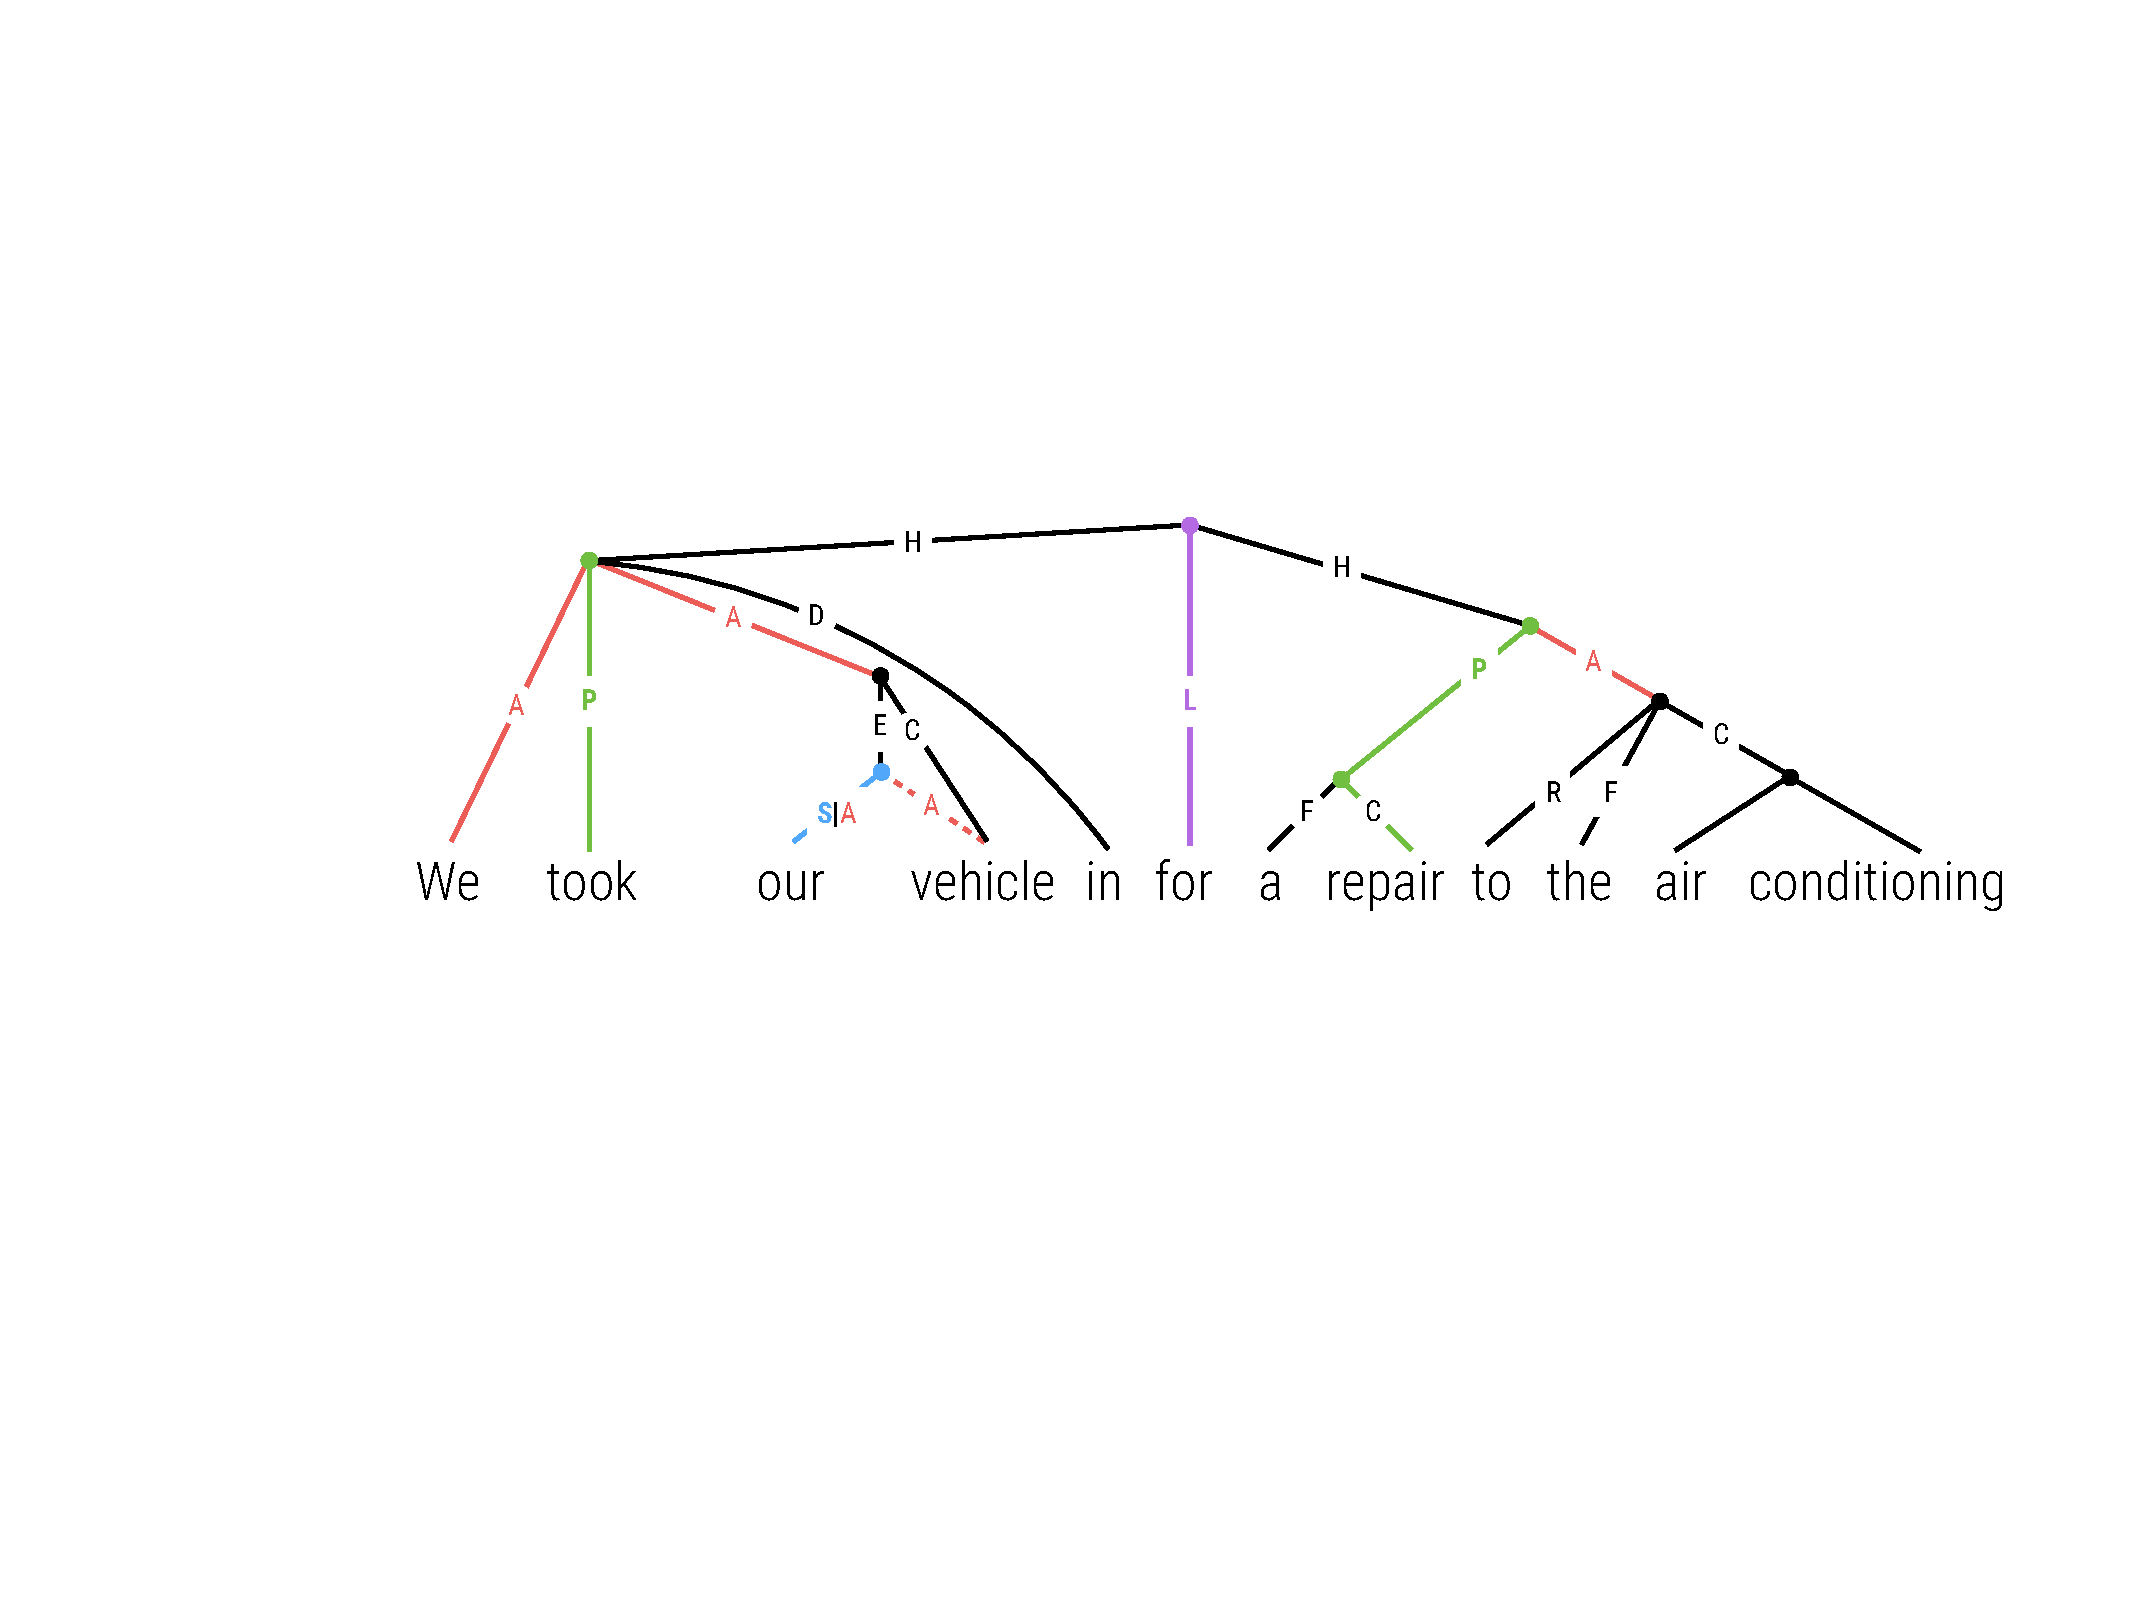
\includegraphics[width=\textwidth]{ex-ucca.pdf}
% \end{frame}
% \section{Guidelines}
% \section{Data}
% \section{Extensions}


% \begin{frame}
% \frametitle{Extensions}
%     \begin{itemize}
%         \item ``UCCA is built as a multi-layered structure, which allows for its open-ended extension.'' \citep{abend2013universal}
%         \item Foundational layer has relatively flat structure, makes coarse distinctions
%         \item Additional layers can capture additional semantic phenomena by...
%         \begin{itemize}
%             \item refining existing categories
%             \item introducing new distinctions
%             \item adding deeper\slash more complex structure
%         \end{itemize}
%     \end{itemize}
% \end{frame}

% \begin{frame}
% \frametitle{Extensions: Semantic Roles}
%     \begin{itemize}
%         \item Labeling all participants as `Participant' does not answer the classic `WDWTW?' (Who did what to whom?)
%         \item We need semantic (thematic, theta) roles: \{Agent, Theme, Experiencer, ...\}
%         \item Option 1: Refine all Participants with a semantic role
%         \item Option 2: Annotate all semantic roles explicitly marked with a lexical item
%     \end{itemize}
% \end{frame}

% \begin{frame}
% \frametitle{Extensions: Semantic Roles}
%     \begin{itemize}
%         \item Option 1: Refine all Participants with a semantic role
%         \item \citet{shalev-etal-2019-preparing}
%         \item ... (summarize process and findings)
%     \end{itemize}
% \end{frame}

% \begin{frame}
% \frametitle{Extensions: Semantic Roles}
%     \begin{itemize}
%         \item Option 2: Annotate all semantic roles explicitly marked with a lexical item
%         \item \citet{prange2019made}
%         \item ... (summarize process and findings, including but not focusing on ML experiments)
%     \end{itemize}
% \end{frame}

% \begin{frame}
% \frametitle{Extensions: Coreference}
%     \begin{itemize}
%         \item \citet{prange2019semantically}
%         \item ... (tell story from UCCA perspective)
%         \item ... (in the end mention comparative experiments with GUM, RED, and OntoNotes. can nicely segue into next section?)
%     \end{itemize}
% \end{frame}

% \section{Comparison to Other Frameworks}
% \begin{frame}
% \frametitle{Comparison to Other Frameworks}
%     \begin{itemize}
%         \item Dimensions along which to compare
%         \begin{itemize}
%             \item \citet{koller2019graph} and \citet{prange2019semantically} taxonomies
%             \item theoretical foundations
%             \item formal properties
%             \item aims, applications, extensions
%         \end{itemize}
%     \end{itemize}
% \end{frame}

% \begin{frame}
% \frametitle{Comparison to Other Frameworks: AMR}
%     \begin{itemize}
%         \item ...
%     \end{itemize}
% \end{frame}

% \begin{frame}
% \frametitle{Comparison to Other Frameworks: Syntactic Representation}
%     \begin{itemize}
%         \item ...
%     \end{itemize}
% \end{frame}

% \begin{frame}
% \frametitle{Comparison to Other Frameworks: Discourse Representation}
%     \begin{itemize}
%         \item ...
%     \end{itemize}
% \end{frame}

% \begin{frame}
% \frametitle{Comparison to Other Frameworks: MRP Shared Task}
%     \begin{itemize}
%         \item introduce goals, tools, and findings of MRP shared task
%         \item coarsely compare UCCA with PTG, EDS, DRG
%     \end{itemize}
% \end{frame}

\section{Parsing}


\begin{frame}
\frametitle{UCCA Parsing}
{\Large \textbf{The Task:} Given plain text,
predict its UCCA graph representation.}

\vfill

\begin{center}
    {\rmfamily\small They thought about taking a short break}
\[\Downarrow\]
\scalebox{.75}{
\begin{tikzpicture}[level distance=16mm, sibling distance=28mm, ->, thick,
  level 2/.style={sibling distance=12mm},
  level 3/.style={sibling distance=18mm},
  edge from parent/.append style={nodes={font=\scriptsize}}]
  \tikzstyle{word} = [font=\rmfamily,color=black]
    \node (ROOT) [fill=blue, circle] {}
      child {node (They) [word] {They} edge from parent node[midway, fill=white] {A}}
      child {node [word] {thought} edge from parent node[midway, fill=white] {P}}
      child {node (abouttakingashortbreak) [fill=blue, circle] {}
      {
        child {node [word] {about} edge from parent node[midway, fill=white] {R}}
        child {node (takingabreak) [fill=blue, circle] {}
        {
          child {node [word] {taking} edge from parent node[midway, fill=white] {F}}
          child {node [word] {a} edge from parent node[midway, fill=white] {F}}
          child {node [word] (short) {short} edge from parent[draw=none]}
          child {node [word] {break} edge from parent node[midway, fill=white] {C}}
        } edge from parent node[midway, fill=white] {P} }
      } edge from parent node[midway, fill=white] {A} }
      ;
    \draw[bend left,dashed,->] (abouttakingashortbreak) to node [auto] {\scriptsize A} (They);
    \draw[bend left,->] (abouttakingashortbreak) to node [auto] {\scriptsize D} (short);
\end{tikzpicture}}
\end{center}
\end{frame}

\begin{frame}
\frametitle{Graph Structure}
Labeled directed acyclic graphs (DAGs).
Complex units are {\color{blue} non-terminal nodes}.
\onslide<2->{
  Phrases may be {\color{red} discontinuous}.
}

\onslide<3->{
  \textit{Remote edges} enable {\color{orange} reentrancy}.
}

\hspace*{33mm}
\begin{tikzpicture}[level distance=16mm, sibling distance=18mm, ->, thick,
  level 2/.style={sibling distance=12mm},
  level 3/.style={sibling distance=11mm},
  edge from parent/.append style={nodes={font=\scriptsize}}]
  \tikzstyle{word} = [font=\rmfamily,color=black]
    \node (ROOT) [fill=blue, circle] {}
      child {node (They) [word] {They} edge from parent node[midway, fill=white] {A}}
      child {node [word] {thought} edge from parent node[midway, fill=white] {P}}
      child {node (abouttakingashortbreak) [fill=blue, circle] {}
      {
        child {node [word] {about} edge from parent node[midway, fill=white] {R}}
        child {node (takingabreak) [fill=blue, circle] {}
        {
          child {node [word] {taking} edge from parent node[midway, fill=white] {F}}
          child {node [word] {a} edge from parent node[midway, fill=white] {F}}
          child {node [word] (short) {short} edge from parent[draw=none]}
          child {node [word] {break} edge from parent node[midway, fill=white] {C}}
        } edge from parent node[midway, fill=white] {P} }
      } edge from parent node[midway, fill=white] {A} }
      ;
    \draw[bend left,dashed,->,visible on=<-2>] (abouttakingashortbreak) to node [auto] {\scriptsize A} (They);
    \draw[bend left,dashed,->,orange,very thick,visible on=<3->] (abouttakingashortbreak) to node [auto] {\scriptsize A} (They);
    \draw[bend left,->,visible on=<1>] (abouttakingashortbreak) to node [auto] {\scriptsize D} (short);
    \draw[bend left,->,visible on=<3->] (abouttakingashortbreak) to node [auto] {\scriptsize D} (short);
    \draw[bend left,->,red,very thick,visible on=<2>] (abouttakingashortbreak) to node [auto] {\scriptsize D} (short);
    \node[visible on=<3->] at (3.5,-.4) {----- primary edge};
    \node[visible on=<3->] at (3.5,-1.4) {- - - remote edge};
\end{tikzpicture}

\onslide<2->{
  \vspace{-54mm}\normalsize
  \begin{adjustbox}{margin=1pt,frame}
  \begin{tabular}{>{\ttfamily}c@{\hskip 5mm\bfseries}l}
    A & Participant \\
    C & Center \\
    D & Adverbial \\
    E & Elaborator \\
    F & Function \\
    G & Ground \\
    H & Parallel scene \\
    L & Linker \\
    P & Process \\
    R & Relator \\
    S & State \\
    U & Punctuation
  \end{tabular}
  \end{adjustbox}
}
\end{frame}

\begin{frame}
\frametitle{Data Statistics}
\centering
\def\arraystretch{1.5}
\scalebox{.7}{
\begin{tabular}{l|r|rrr|r}
    & \multicolumn{1}{c|}{Wiki} & \multicolumn{3}{c|}{20K} & \multicolumn{1}{c}{EWT} \\
    & \multicolumn{1}{c|}{en} & \multicolumn{1}{c}{en} & \multicolumn{1}{c}{fr} & \multicolumn{1}{c|}{de} & \multicolumn{1}{c}{en} \\
    \hline
    \# sentences&5,141&492&492&6,514&3,813 \\
    \# tokens&158K&12K&12K&144K&55K \\
    \hline
    \# {\color{blue} non-terminal nodes}&62,002&4,699&5,110&51,934&18,156 \\
    \% {\color{red}discontinuous}&1.71&3.19&4.64&8.87&3.87 \\
    \% {\color{orange}reentrant}&1.84&0.89&0.65&0.31&0.83 \\
    \hline
    \# edges&208,937&16,803&17,520&187,533&60,739 \\
    \% primary&97.40&96.79&97.02&97.32&97.32 \\
    \% remote&2.60&3.21&2.98&2.68&2.68
\end{tabular}
}
\end{frame}

\subsection{TUPA}

\begin{frame}
\frametitle{Transition-based UCCA Parser}
\textit{A Transition-Based Directed Acyclic Graph Parser for UCCA} \citep{hershcovich2017a}.
\vfill

\centering
\scalebox{.7}{
\begin{tikzpicture}[level distance=15mm, sibling distance=2cm, ->, thick,
    every node/.append style={font=\rmfamily},
    edge from parent path={(\tikzparentnode.center) -- (\tikzchildnode.north)}]
    \node(ROOT)[fill=black, circle] at (3,0) {}
      child {node (They) {They} edge from parent node [left] {A}}
      child {node (thought) {thought} edge from parent node [left] {P}}
      child {node (abouttakingashortbreak) [fill=blue, circle] {} 
      { 
        child {node (to) {about} edge from parent node [right] {R}}
        child {node (takingabreak) [fill=red, circle] {}
        {
          child {node (take) {taking} edge from parent node [above] {F}}      
          child {node (a) {a} edge from parent node [right] {F}} 
          child {node (short) {short} edge from parent [draw=none]}
          child {node (break) {break} edge from parent node [above] {C}}  
        } edge from parent [draw=none]}
      } edge from parent [draw=none]}
      ;
    \draw(abouttakingashortbreak) to node [left] {P} (takingabreak); 
    \draw(ROOT) to node [left] {A} (abouttakingashortbreak);
    \draw[bend left,dashed] (abouttakingashortbreak) to node [auto] {A} (They);
    \draw[bend left] (abouttakingashortbreak) to node [auto] {D} (short);
\end{tikzpicture}}
\[\Updownarrow\]
\begin{flushleft}
\footnotesize
\textsc{Shift}, \textsc{Right-Edge$_A$}, \textsc{Shift}, \textsc{Swap}, \textsc{Right-Edge$_P$}, \textsc{Reduce}, \textsc{Shift}, \textsc{Shift}, \textsc{Node$_R$}, \textsc{Reduce}, \textsc{Left-Remote$_A$}, \textsc{Shift}, \textsc{Shift}, \textsc{Node$_C$}, \textsc{Reduce}, \textsc{Shift}, \textsc{Right-Edge$_P$}, \textsc{Shift}, \textsc{Right-Edge$_F$}, \textsc{Reduce}, \textsc{Shift}, \textsc{Swap}, \textsc{Right-Edge$_D$}, \textsc{Reduce}, \textsc{Swap}, \textsc{Right-Edge$_A$}, \textsc{Reduce}, \textsc{Reduce}, \textsc{Shift}, \textsc{Reduce}, \textsc{Shift}, \textsc{Right-Edge$_C$}, \textsc{Finish}
\end{flushleft}
\end{frame}

\begin{frame}
\frametitle{Transition-based UCCA Parser}

Parses text $w_1 \ldots w_n$ to graph $G$ incrementally by applying transitions to the parser state,
consisting of: stack, buffer and constructed graph.

\pause
\vfill
Initial state:
\scalebox{.8}{
\begin{tikzpicture}[xscale=1.4,every node/.append style={font=\rmfamily,
                    anchor=west,text height=.6ex,text depth=0}, circle]
    \draw[xstep=1,ystep=.5,color=gray] (-.01,0) grid (1,.5);
    \node[style={font=\sffamily}] at (-.1,.8) {stack};
    \node[fill=black] at (.3,.25) {};
    \draw[xstep=1,ystep=.5,color=gray] (2,0) grid (9,.5);
    \node[style={font=\sffamily}] at (8,.8) {buffer};
    \node at (2,.2) {\small They};
    \node at (3,.2) {\small thought};
    \node at (4,.2) {\small about};
    \node at (5,.2) {\small taking};
    \node at (6,.2) {\small a};
    \node at (7,.2) {\small short};
    \node at (8,.2) {\small break};
\end{tikzpicture}}

\vfill
\pause
Transitions:

\{\textsc{Shift, Reduce, {\color{blue}Node$_X$}, Left-Edge$_X$, Right-Edge$_X$,}\\
\hspace{5mm}\textsc{{\color{orange}Left-Remote$_X$}, {\color{orange}Right-Remote$_X$}, {\color{red}Swap}, Finish}\}
\end{frame}

\begin{frame}
\frametitle{Example: TUPA Transition Sequence}
\begin{minipage}[t][8mm][t]{\textwidth}
    $\Rightarrow$\textsc{
        \only<1>{Shift}\only<2>{Right-Edge$_A$}\only<3>{Shift}\only<4>{Swap}\only<5>{Right-Edge$_P$}\only<6>{Reduce}\only<7>{Shift}\only<8>{Shift}\only<9>{Node$_R$}\only<10>{Reduce}\only<11>{Shift}\only<12>{Left-Remote$_A$}\only<13>{Shift}\only<14>{Node$_C$}\only<15>{Reduce}\only<16>{Shift}\only<17>{Right-Edge$_P$}\only<18>{Shift}\only<19>{Right-Edge$_F$}\only<20>{Reduce}\only<21>{Shift}\only<22>{Swap}\only<23>{Right-Edge$_D$}\only<24>{Reduce}\only<25>{Swap}\only<26>{Right-Edge$_A$}\only<27>{Reduce}\only<28>{Reduce}\only<29>{Shift}\only<30>{Reduce}\only<31>{Shift}\only<32>{Right-Edge$_C$}\only<33>{Finish}
    }
\end{minipage}

\vfill

\scalebox{.8}{
\begin{tikzpicture}[xscale=1.4,every node/.append style={font=\rmfamily, thick,
                    anchor=west,text height=.6ex,text depth=0}]
    \begin{scope}[style={font=\sffamily}]
      \node at (-.1,.8) {stack};
      \node at (8,  .8) {buffer};
    \end{scope}
    \begin{scope}[xstep=1,ystep=.5,color=red,line width=1pt]
      \only<31>    \draw (-.01,0) grid (1,.5);
      \only<1,7>   \draw (.99, 0) grid (2,.5);
      \only<2,5,26>\draw (-.01,0) grid (2,.5);
      \only<3,8,11>\draw (1.99,0) grid (3,.5);
      \only<13,16> \draw (2.99,0) grid (4,.5);
      \only<18,21> \draw (3.99,0) grid (5,.5);
      \only<17>    \draw (1.99,0) grid (4,.5);
      \only<19>    \draw (2.99,0) grid (5,.5);
      \only<4>     \draw (3,   0) grid (4,.5);
      \only<9>     \draw (4,   0) grid (5,.5);
      \only<14>    \draw (5,   0) grid (6,.5);
      \only<22>    \draw (7,   0) grid (8,.5);
      \only<25>    \draw (6,   0) grid (7,.5);
      \only<23>    \draw (1.99,0) grid (4,.5);
      \only<32>    \draw (-.01,0) grid (2,.5);
      \only<12>    \draw (.99, 0) grid (3,.5);
    \end{scope}
    \begin{scope}[xstep=1,ystep=.5,color=gray]
      \only<6,27,29,31->         \draw (-.01,0) grid (1, .5);
      \only<-2,4-5,7,10,25-26,33>\draw (-.01,0) grid (2, .5);
      \only<3,8-9,11-12,15,24>   \draw (-.01,0) grid (3, .5);
      \only<13-14,16-17,20,22-23>\draw (-.01,0) grid (4, .5);
      \only<18-19,21>            \draw (-.01,0) grid (5, .5);
      \only<-2,4-6>              \draw (3,   0) grid (9,.5);
      \only<3,5-7,9-10>          \draw (4,   0) grid (9,.5);
      \only<8,11-12,14-15>       \draw (5,   0) grid (9,.5);
      \only<13,16-17,25-28>      \draw (6,   0) grid (9,.5);
      \only<18-20,22-24,29-30>   \draw (7,   0) grid (9,.5);
      \only<21,31>               \draw (8,   0) grid (9,.5);
    \end{scope}
    \begin{scope}[xstep=.1,ystep=.5,color=gray]
      \only<28,30> \draw (-.01,0) grid (.1,.5);
      \only<32->   \draw (8.89,0) grid (9.01,.5);
    \end{scope}
    \only<-27>      \node[fill=black, circle] at (.3, .25) {};
    \only<25-26>    \node[fill=blue,  circle] at (1.3,.25) {};
    \only<11-24>    \node[fill=blue,  circle] at (2.3,.25) {};
    \only<31->      \node[fill=red,   circle] at (.3, .25) {};
    \only<16-21>    \node[fill=red,   circle] at (3.3,.25) {};
    \only<9-10>     \node[fill=blue,  circle] at (4.3,.25) {};
    \only<14-15>    \node[fill=red,   circle] at (5.3,.25) {};
    \only<22-30>    \node[fill=red,   circle] at (7.3,.25) {};
    \only<29>       \node at (0,.2) {\small They};
    \only<1-3,7-24> \node at (1,.2) {\small They};
    \only<4-5>      \node at (1,.2) {\small thought};
    \only<3>        \node at (2,.2) {\small thought};
    \only<8-9>      \node at (2,.2) {\small about};
    \only<13-14>    \node at (3,.2) {\small taking};
    \only<18-19>    \node at (4,.2) {\small a};
    \only<21>       \node at (4,.2) {\small short};
    \only<22-23>    \node at (3,.2) {\small short};
    \only<32->      \node at (1,.2) {\small break};
    \only<4-6>      \node at (3,.2) {\small They};
    \only<25-28>    \node at (6,.2) {\small They};
    \only<-2>       \node at (3,.2) {\small thought};
    \only<-7>       \node at (4,.2) {\small about};
    \only<-12>      \node at (5,.2) {\small taking};
    \only<-17>      \node at (6,.2) {\small a};
    \only<-20>      \node at (7,.2) {\small short};
    \only<-31>      \node at (8,.2) {\small break};
\end{tikzpicture}}
\vfill
\fbox{
\begin{tikzpicture}[level distance=14mm, sibling distance=21mm, ->,
    every node/.append style={font=\rmfamily},
    edge from parent/.append style={nodes={font=\scriptsize}},
    edge from parent path={(\tikzparentnode.center) -- (\tikzchildnode.north)}]
    \node[anchor=west,style={font=\sffamily}] at (0,0) {graph};
    \node(ROOT)[fill=black, circle, visible on=<1->] at (3,0) {}
      child [visible on=<2->,alt=<2>{draw=red}{}] {node (They) {They} edge from parent node [left] {A}}
      child [visible on=<5->,alt=<5>{draw=red}{}] {node (thought) {thought} edge from parent node [left] {P}}
      child [visible on=<9->] {node (abouttakingashortbreak) [fill=blue, circle] {}
      {
        child [visible on=<9->,alt=<9>{draw=red}{}] {node (to) {about} edge from parent node [right] {R}}
        child [visible on=<14->] {node (takingabreak) [fill=red, circle] {}
        {
          child [visible on=<14->] {node (take) {taking} edge from parent node [above] {F}}
          child [visible on=<19->,alt=<19>{draw=red}{}] {node (a) {a} edge from parent node [right] {F}}
          child [visible on=<23->,alt=<23>{draw=red}{}] {node (short) {short} edge from parent [draw=none]}
          child [visible on=<32->,alt=<32>{draw=red}{}] {node (break) {break} edge from parent node [above] {C}}
        } edge from parent [draw=none]}
      } edge from parent [draw=none]}
      ;
    \draw[visible on=<17->,alt=<17>{draw=red}{}] (abouttakingashortbreak) to node [left] {\scriptsize P} (takingabreak);
    \draw[visible on=<26->,alt=<26>{draw=red}{}] (ROOT) to node [left] {\scriptsize A} (abouttakingashortbreak);
    \draw[bend left,dashed, visible on=<12->,alt=<12>{draw=red}{}] (abouttakingashortbreak) to node [auto] {\scriptsize A} (They);
    \draw[bend left, visible on=<23->,alt=<23>{draw=red}{}] (abouttakingashortbreak) to node [auto] {\scriptsize D} (short);
\end{tikzpicture}}
\end{frame}

\begin{frame}
\frametitle{TUPA model}
Learns to predict next transition based on current state.

\centering
\fbox{\scalebox{.65}{
\begin{minipage}{.65\textwidth}
\begin{tikzpicture}[xscale=1.3,every node/.append style={font=\rmfamily}]
    \node[anchor=west,style={font=\sffamily}] at (-1,.25){stack};
    \draw[xstep=1,ystep=.5,color=gray] (-.01,0) grid (4,.5);
    \node[fill=black, circle] at (.5,.25) {};
    \node[fill=blue, circle] at (2.5,.25) {};
    \node[anchor=west] at (1,.25) {\small They};
    \node[anchor=west] at (3,.25) {\small taking};
\end{tikzpicture}

\vspace{1cm}
\begin{tikzpicture}[xscale=1.3,every node/.append style={font=\rmfamily}]
    \node[anchor=west,style={font=\sffamily}] at (-1,.25){buffer};
    \draw[xstep=1,ystep=.5,color=gray] (-.01,0) grid (4,.5);
    \node[fill=red, circle] at (.5,.25) {};
    \node[anchor=west] at (1,.25) {\small a};
    \node[anchor=west] at (2,.25) {\small short};
    \node[anchor=west] at (3,.25) {\small break};
\end{tikzpicture}
\end{minipage}
\begin{minipage}{.4\textwidth}
\scalebox{.6}{
\begin{tikzpicture}[xscale=1.5,level distance=1cm, sibling distance=12mm, ->,
    every node/.append style={font=\rmfamily,
                    anchor=west,text height=.6ex,text depth=0},
    edge from parent/.append style={nodes={font=\scriptsize}},
    edge from parent path={(\tikzparentnode.center) -- (\tikzchildnode.north)}]
    \node[anchor=west,style={font=\sffamily}] at (3,0) {graph};
    \draw[color=gray] (.2,.3) rectangle (3.9,-3.2);
    \node(ROOT)[fill=black, circle] at (1.2,0) {}
      child {node (They) {They} edge from parent node [left] {A}}
      child {node {thought} edge from parent node [left] {P}}
      child {node (abouttakingashortbreak) [fill=blue, circle] {}
      {
        child {node {about} edge from parent node [left] {R}}
        child {node (takingabreak) [fill=red, circle] {}
        {
          child {node {taking} edge from parent node [above] {F}}
          child [opacity=0] {node {a} edge from parent node [right] {F}}
          child [opacity=0] {node (short) {short} edge from parent [draw=none]}
          child [opacity=0] {node {break} edge from parent node [right] {C}}
        } edge from parent [draw=none]}
      } edge from parent [draw=none]}
      ;
\end{tikzpicture}
}
\end{minipage}
}}

\scalebox{.65}{
\begin{tikzpicture}[->,every node/.append style={anchor=north,text height=2ex,text depth=0}]
    \tiny
    \tikzstyle{main}=[circle, minimum size=7mm, draw=black!80, node distance=12mm]
    \foreach \i/\word in {1/{They},3/{thought},5/{about},7/{taking},9/{a},11/{short},13/{break}} {
        \node (x\i) at (\i,-1.3) {\Large\textrm\word};
        \node[main, fill=white!100] (h\i) at (\i,0) {};
        \path (x\i) edge (h\i);
        \node[main, fill=white!100] (i\i) at (\i.5,.8) {};
        \path (x\i) edge [bend right] (i\i);
        \node[main, fill=white!100] (l\i) at (\i.5,2.3) {};
        \path (h\i) edge [bend left] (l\i);
        \path (i\i) edge (l\i);
        \node[main, fill=white!100] (k\i) at (\i,3.1) {};
        \path (i\i) edge [bend left] (k\i);
        \path (h\i) edge [bend left] (k\i);
    }
    \foreach \current/\next in {1/3,3/5,5/7,7/9,9/11,11/13} {
        \path (h\current) edge (h\next);
        \path (i\next) edge (i\current);
        \path (l\current) edge (l\next);
        \path (k\next) edge (k\current);
    }
    \node[main, fill=white!100] (mlp) at (7,4.6) {};
    \foreach \i in {1,5,7,9} {
        \path (l\i) edge (mlp);
        \path (k\i) edge (mlp);
    }
    \coordinate (state) at (10.5,6.5);
    \path (state) edge [bend left] (mlp);
    \node (transition) at (7,5.8) {\large\textsc{Node}$_C$};
    \path (mlp) edge (transition);
\end{tikzpicture}
}
\end{frame}

\begin{frame}
\frametitle{Training}
An \textit{oracle} provides the transition sequence given the correct graph:

\vfill

\centering
\scalebox{.7}{
\begin{tikzpicture}[level distance=15mm, sibling distance=2cm, ->, thick,
    every node/.append style={font=\rmfamily},
    edge from parent path={(\tikzparentnode.center) -- (\tikzchildnode.north)}]
    \node(ROOT)[fill=black, circle] at (3,0) {}
      child {node (They) {They} edge from parent node [left] {A}}
      child {node (thought) {thought} edge from parent node [left] {P}}
      child {node (abouttakingashortbreak) [fill=blue, circle] {} 
      { 
        child {node (to) {about} edge from parent node [right] {R}}
        child {node (takingabreak) [fill=red, circle] {}
        {
          child {node (take) {taking} edge from parent node [above] {F}}      
          child {node (a) {a} edge from parent node [right] {F}} 
          child {node (short) {short} edge from parent [draw=none]}
          child {node (break) {break} edge from parent node [above] {C}}  
        } edge from parent [draw=none]}
      } edge from parent [draw=none]}
      ;
    \draw(abouttakingashortbreak) to node [left] {P} (takingabreak); 
    \draw(ROOT) to node [left] {A} (abouttakingashortbreak);
    \draw[bend left,dashed] (abouttakingashortbreak) to node [auto] {A} (They);
    \draw[bend left] (abouttakingashortbreak) to node [auto] {D} (short);
\end{tikzpicture}}
\[\Updownarrow\]
\begin{flushleft}
\footnotesize
\textsc{Shift}, \textsc{Right-Edge$_A$}, \textsc{Shift}, \textsc{Swap}, \textsc{Right-Edge$_P$}, \textsc{Reduce}, \textsc{Shift}, \textsc{Shift}, \textsc{Node$_R$}, \textsc{Reduce}, \textsc{Left-Remote$_A$}, \textsc{Shift}, \textsc{Shift}, \textsc{Node$_C$}, \textsc{Reduce}, \textsc{Shift}, \textsc{Right-Edge$_P$}, \textsc{Shift}, \textsc{Right-Edge$_F$}, \textsc{Reduce}, \textsc{Shift}, \textsc{Swap}, \textsc{Right-Edge$_D$}, \textsc{Reduce}, \textsc{Swap}, \textsc{Right-Edge$_A$}, \textsc{Reduce}, \textsc{Reduce}, \textsc{Shift}, \textsc{Reduce}, \textsc{Shift}, \textsc{Right-Edge$_C$}, \textsc{Finish}
\end{flushleft}
\end{frame}



\begin{frame}
\frametitle{TUPA Model}
Learns to greedily predict transition based on current state.

\only<1>{

\vspace{1cm}

Features include:

\{words, parts of speech, syntactic dependencies, existing edge labels\} \\
from the stack and buffer + parents, children, grandchildren.

\vspace{5mm}
\begin{tikzpicture}
    \draw[xstep=1cm,ystep=5mm,color=gray] (-.01,0) grid (4,.5);
    \draw[xstep=1cm,ystep=5mm,color=gray] (5,0) grid (10,.5);
    \node[anchor=west] at (-.1,1) {stack};
    \node[anchor=west] at (8.9,1) {buffer};
    \foreach \i in {0.5,8.5,9.5} {
        \node[fill=gray, circle] at (\i,.25) {};
    }
    \foreach \i in {1.5,2.5,3.5,5.5,6.5,7.5} {
        \node[fill=black, circle] at (\i,.25) {};
    }
\end{tikzpicture}
}

\pause

\centering
\fbox{\scalebox{.65}{
\begin{minipage}{.6\textwidth}
\begin{tikzpicture}[xscale=1.3,every node/.append style={font=\rmfamily}]
    \node[anchor=west,style={font=\sffamily}] at (-1,.25){stack};
    \draw[xstep=1,ystep=.5,color=gray] (-.01,0) grid (4,.5);
    \node[fill=black, circle] at (.5,.25) {};
    \node[fill=blue, circle] at (2.5,.25) {};
    \node[anchor=west] at (1,.25) {\small They};
    \node[anchor=west] at (3,.25) {\small taking};
\end{tikzpicture}

\vspace{1cm}
\begin{tikzpicture}[xscale=1.3,every node/.append style={font=\rmfamily}]
    \node[anchor=west,style={font=\sffamily}] at (-1,.25){buffer};
    \draw[xstep=1,ystep=.5,color=gray] (-.01,0) grid (4,.5);
    \node[fill=red, circle] at (.5,.25) {};
    \node[anchor=west] at (1,.25) {\small a};
    \node[anchor=west] at (2,.25) {\small short};
    \node[anchor=west] at (3,.25) {\small break};
\end{tikzpicture}
\end{minipage}
\begin{minipage}{.4\textwidth}
\scalebox{.65}{
\begin{tikzpicture}[xscale=1.5,level distance=1cm, sibling distance=12mm, ->,
    every node/.append style={font=\rmfamily,
                    anchor=west,text height=.6ex,text depth=0},
    edge from parent/.append style={nodes={font=\scriptsize}},
    edge from parent path={(\tikzparentnode.center) -- (\tikzchildnode.north)}]
    \node[anchor=west,style={font=\sffamily}] at (3,0) {graph};
    \draw[color=gray] (.2,.3) rectangle (3.9,-3.2);
    \node(ROOT)[fill=black, circle] at (1.2,0) {}
      child {node (They) {They} edge from parent node [left] {A}}
      child {node {thought} edge from parent node [left] {P}}
      child {node (abouttakingashortbreak) [fill=blue, circle] {}
      {
        child {node {about} edge from parent node [left] {R}}
        child {node (takingabreak) [fill=red, circle] {}
        {
          child {node {taking} edge from parent node [above] {F}}
          child [opacity=0] {node {a} edge from parent node [right] {F}}
          child [opacity=0] {node (short) {short} edge from parent [draw=none]}
          child [opacity=0] {node {break} edge from parent node [right] {C}}
        } edge from parent [draw=none]}
      } edge from parent [draw=none]}
      ;
\end{tikzpicture}
}
\end{minipage}
}}

\scalebox{.65}{
\begin{tikzpicture}[->,every node/.append style={anchor=north,text height=2ex,text depth=0}]
    \tiny
    \tikzstyle{main}=[circle, minimum size=7mm, draw=black!80, node distance=12mm]
    \foreach \i/\word in {1/{They},3/{thought},5/{about},7/{taking},9/{a},11/{short},13/{break}} {
        \node (x\i) at (\i,-1.3) {\Large\textrm\word};
        \node[main, fill=white!100] (h\i) at (\i,0) {LSTM};
        \path (x\i) edge (h\i);
        \node[main, fill=white!100] (i\i) at (\i.5,.8) {LSTM};
        \path (x\i) edge [bend right] (i\i);
        \node[main, fill=white!100] (l\i) at (\i.5,2.3) {LSTM};
        \path (h\i) edge [bend left] (l\i);
        \path (i\i) edge (l\i);
        \node[main, fill=white!100] (k\i) at (\i,3.1) {LSTM};
        \path (i\i) edge [bend left] (k\i);
        \path (h\i) edge [bend left] (k\i);
    }
    \foreach \current/\next in {1/3,3/5,5/7,7/9,9/11,11/13} {
        \path (h\current) edge (h\next);
        \path (i\next) edge (i\current);
        \path (l\current) edge (l\next);
        \path (k\next) edge (k\current);
    }
    \node[main, fill=white!100] (mlp) at (7,4.6) {MLP};
    \foreach \i in {1,5,7,9} {
        \path (l\i) edge (mlp);
        \path (k\i) edge (mlp);
    }
    \coordinate (state) at (10.5,6.5);
    \path (state) edge [bend left] (mlp);
    \node (transition) at (7,5.8) {\large\textsc{Node}$_C$};
    \path (mlp) edge (transition);
\end{tikzpicture}
}
\end{frame}

\begin{frame}
\frametitle{Comparing to Existing Methods}
Using conversion-based approximation as baseline, \\
with bi-lexical DAG parsers and transition-based tree parsers.

\vfill
\begin{center}
    \begin{dependency}
    \begin{deptext}[column sep=.5em,ampersand replacement=\^,font=\rmfamily, thick]
	They \^ thought \^ about \^ taking \^ a \^ short \^ break \\
    \end{deptext}
    \depedge{2}{1}{A}
    \depedge[dashed,edge start x offset=6pt,edge end x offset=-6pt,edge unit distance=3.5ex]{7}{1}{A}
    \depedge{7}{3}{R}
    \depedge{7}{4}{F}
    \depedge{7}{5}{F}
    \depedge{7}{6}{D}
    \depedge{2}{7}{A}
    \end{dependency}
    \captionof{figure}{UCCA bi-lexical DAG approximation.}
\end{center}
\end{frame}


\begin{frame}
\frametitle{Bi-lexical Graph Approximation}
\begin{enumerate}
 \item Convert UCCA to bi-lexical DAGs.
 \item Train bi-lexical parsers.
 \item Parse test set.
 \item Convert to UCCA.
 \item Evaluate.
\end{enumerate}

\vspace{-15mm}

\begin{minipage}{.225\textwidth}
  \vspace{1cm}
  \begin{flushright}
    \begin{tikzpicture}[<->]
      \draw [ultra thick,red] (1,1) to[out=180,in=90] (0,0);
    \end{tikzpicture}
  \end{flushright}
\end{minipage}
\begin{minipage}{.5\textwidth}
    \begin{tikzpicture}[level distance=13mm, sibling distance=17mm, ->, thick,
        every circle node/.append style={fill=black},
        edge from parent/.append style={nodes={font=\scriptsize}},
        edge from parent path={(\tikzparentnode.center) -- (\tikzchildnode.north)}]
      \tikzstyle{word} = [font=\rmfamily,color=black]
      \node (ROOT) [circle] {}
        child {node (After) [word] {After} edge from parent node[left] {L}}
        child {node (graduation) [circle] {}
        {
          child {node [word] {graduation} edge from parent node[left] {P}}
        } edge from parent node[left] {H} }
        child {node [word] {,} edge from parent node[right] {U}}
        child {node (moved) [circle] {}
        {
          child {node (John) [word] {John} edge from parent node[left] {A}}
          child {node [word] {moved} edge from parent node[left] {P}}
          child {node [circle] {}
          {
            child {node [word] {to} edge from parent node[left] {R}}
            child {node [word] {Copenhagen} edge from parent node[right] {C}}
          } edge from parent node[right] {A} }
        } edge from parent node[right] {H} }
        ;
      \draw[dashed,->] (graduation) to node [auto] {\scriptsize A} (John);
    \end{tikzpicture}
\end{minipage}

\vspace{-14mm}
\begin{flushleft}
    \begin{dependency}
    \begin{deptext}[column sep=.7em,ampersand replacement=\^,font=\rmfamily, thick]
	After \^ graduation \^ , \^ John \^ moved \^ to \^ Copenhagen \\
    \end{deptext}
    \depedge{2}{1}{L}
    \depedge{2}{3}{U}
    \depedge[dashed]{2}{4}{A}
    \depedge{5}{4}{A}
    \depedge{2}{5}{H}
    \depedge{7}{6}{R}
    \depedge{5}{7}{A}
    \end{dependency}
\end{flushleft}
\end{frame}


\begin{frame}
    \frametitle{Meaning Representations}

      \begin{flushright}
        \scalebox{.4}{
\begin{tikzpicture}[level distance=2cm, sibling distance=25mm, ->, draw=Indigo, thick]
    \node[font=\bf\sffamily\Huge,Indigo] at (-3,0) {UCCA};
    \node (ROOT) [fill=Indigo, circle] {}
      child {node (After) {After} edge from parent node[left] {L\;}}
      child {node (graduation) [fill=Indigo, circle] {}
      {
        child {node {graduation} edge from parent node[left] {P}}
      } edge from parent node[left] {H} }
      child {node {,} edge from parent node[right] {U}}
      child {node (moved) [fill=Indigo, circle] {}
      {
        child {node (Daniel) {Daniel} edge from parent node[left] {A}}
        child {node {moved} edge from parent node[left] {P}}
        child {node [fill=Indigo, circle] {}
        {
          child {node {to} edge from parent node[left] {R}}
          child {node {Copenhagen} edge from parent node[left] {C}}
        } edge from parent node[left] {A} }
      } edge from parent node[right] {H} }
      ;
    \draw[dashed,->] (graduation) to node [auto] {A} (Daniel);
\end{tikzpicture}
        }
      \end{flushright}
    
    \vspace{-23mm}
    
    \scalebox{.4}{
\begin{tikzpicture}[thick]
\node[font=\bf\sffamily\Huge,DarkGreen] at (0,6) {AMR};
\graph[layered layout, sibling distance=4cm, layer distance=2cm, nodes={ellipse,draw=DarkGreen}, edges={nodes={sloped}, DarkGreen}]{
a4 Copenhagen[as={Copenhagen}];
a2 Daniel[as={Daniel}];
a1[as={person}];
a0[as={move-01}];
a3[as={city}];
a2[as={name}];
a5[as={after}];
a4[as={name}];
a6[as={graduate-01}];

a1 ->  ["name"' above] a2;
a0 ->  ["ARG0"' above] a1;
a0 ->  ["ARG2"' above] a3;
a0 ->  ["time"' above] a5;
a3 ->  ["name"' above] a4;
a2 ->  ["op1"' above] a2 Daniel;
a5 ->  ["op1"' above] a6;
a4 ->  ["op1"' above] a4 Copenhagen;
};
\draw[->, above, DarkGreen] (a6) to node[sloped] {ARG0} (a1);
\end{tikzpicture}
      }
    \vspace{-15mm}
    
    \begin{flushright}
    \begin{minipage}{.01\textwidth}
      \begin{tikzpicture}
        \node[font=\bf\sffamily\Large,DarkRed] {DM};
      \end{tikzpicture}
    \end{minipage}
    \begin{minipage}{.6\textwidth}
        \rmfamily
        \scalebox{.4}{
\begin{dependency}[theme=simple,edge style={-{Latex[length=2mm]}, color=DarkRed},
            text only label, label style={above, color=DarkRed, font=\bf\ttfamily}, font=\small, thick]
    \begin{deptext}[column sep=1em,ampersand replacement=\^]
	After \^ graduation \^ , \^ Daniel \^ moved \^ to \^ Copenhagen \\
    \end{deptext}
    \deproot{5}{top}
    \depedge{1}{2}{ARG2}
    \depedge{1}{5}{ARG1}
    \depedge{5}{4}{ARG1}
    \depedge{6}{5}{ARG1}
    \depedge{6}{7}{ARG2}
\end{dependency}
    }
    \end{minipage}
    \end{flushright}
\end{frame}


\begin{frame}
\frametitle{Syntactic Representations}
    {\color{DarkBlue}\bf\sffamily\Large UD} (Universal Dependencies)
    
    \begin{center}
    \rmfamily
    \begin{dependency}[text only label, edge style={-{Latex[length=2mm]}, color=DarkBlue}, thick,
                       label style={above, color=DarkBlue, font=\bf\ttfamily}, font=\small]
    \begin{deptext}[column sep=.8em,ampersand replacement=\^]
    After \^ graduation \^ , \^ Daniel \^ moved \^ to \^ Copenhagen \\
    \end{deptext}
        \depedge{2}{1}{case}
        \depedge{2}{3}{punct}
        \depedge{5}{4}{nsubj}
        \depedge[edge end x offset=-2pt]{5}{2}{obl}
        \depedge{7}{6}{case}
        \deproot[edge unit distance=2.5ex]{5}{root}
        \depedge{5}{7}{obl}
    \end{dependency}
    \end{center}
\end{frame}


\begin{frame}
    \frametitle{Data}
    \fbox{UCCA training data is scarce}
    \begin{center}
    \begin{minipage}{.15\textwidth}
      (English)
    \end{minipage}
    \begin{minipage}{.7\textwidth}
    \pgfplotstableread[row sep=\\,col sep=&]{
    	corpus & total \\
        \color{DarkBlue} UD & 35791 \\
        \color{DarkRed} DM & 33964 \\
        \color{DarkGreen} AMR & 36521 \\
        \color{Indigo} UCCA & 5141 \\
        }\english
        \begin{tikzpicture}
        \begin{axis}[
        xbar stacked,
        width=10cm,
        height=39mm,
        xmin=0,
        xmax=60000,
        xtick=\empty,
        ytick=data,
        yticklabels from table={\english}{corpus},
        axis x line=none,
        ]
        \addplot [fill=Navy, point meta=explicit symbolic,
        nodes near coords align={anchor=west}] table [x=total,y expr=\coordindex,meta=total] {\english};
        \end{axis}
        \end{tikzpicture}
    \end{minipage}
    \end{center}
    
    \pause
    \vfill
    
    \begin{flushright}
        \fbox{and domains are limited.}
    \end{flushright}
    \begin{center}
    \begin{tabular}{llll}
        \color{Indigo} UCCA  & \color{DarkGreen} AMR  & \color{DarkRed} DM  & \color{NavyBlue} UD  \\
    	Wikipedia & blogs & news & blogs \\ books & news && news \\ reviews & emails && emails \\ & reviews && reviews \\ &&& Q\&A
    \end{tabular}
    \end{center}
\end{frame}

\def\convertedudgraduation{
  \begin{tikzpicture}[level distance=15mm, ->, draw=DarkBlue, thick,
      every node/.append style={sloped,anchor=south,auto=false,font=\scriptsize},
      level 1/.style={sibling distance=16mm},
      level 2/.style={sibling distance=13mm},
      edge from parent path={(\tikzparentnode.center) -- (\tikzchildnode.north)}]
    \tikzstyle{word} = [font=\rmfamily,color=black]
    \node (ROOT) [fill=DarkBlue,circle] {}
      child {node (after) [fill=DarkBlue,circle] {}
      {
        child {node [word] {After{\color{white}g}\quad\quad} edge from parent node {case}}
        child {node [word] {\quad graduation\quad\quad} edge from parent node {head}}
      } edge from parent node {obl}}
      child {node {}
      {
        child {node [word] (comma) {\quad,{\color{white}g}} edge from parent [draw=none]}
      } edge from parent [draw=none]}
      child {node {}
      {
        child {node [word] (Daniel) {Daniel{\color{white}g}} edge from parent [draw=none]}
      } edge from parent [draw=none]}
      child {node {}
      {
        child {node [word] (moved) {moved{\color{white}g}} edge from parent [draw=none]}
      } edge from parent [draw=none]}
      child {node (to) [fill=DarkBlue,circle] {}
      {
          child {node [word] {to{\color{white}g}} edge from parent node {case}}
          child {node [word] {Copenhagen{\color{white}g}} edge from parent node {head}}
      } edge from parent node {obl}}
      ;
      \draw (ROOT) to node {punct} (comma);
      \draw (ROOT) to node {nsubj} (Daniel);
      \draw (ROOT) to node {head} (moved);
  \end{tikzpicture}
}

\begin{frame}
\frametitle{Conversion}
\begin{minipage}{.04\textwidth}
\vspace{4mm}
AMR\\
\vspace{13mm}
SDP\\
\vspace{8mm}
\mbox{CoNLL-U}
\end{minipage}
\begin{minipage}{.44\textwidth}
  \centering
  \scalebox{.55}{
  \begin{tikzpicture}[->,
      every node/.append style={sloped,anchor=south,auto=false,font=\tiny},
      level 1/.style={level distance=14mm,sibling distance=26mm},
      level 2/.style={level distance=13mm},
      level 3/.style={level distance=12mm}]
    \node (ROOT) [draw=black,ellipse] {move-01}
      child {node [draw=black,ellipse] {after}
      {
            child {node (graduation) [draw=black,ellipse] {graduate-01} edge from parent node {op1} }
      } edge from parent node {time} }
      child {node (John) [draw=black,ellipse] {person}
      {
        child {node [draw=black,ellipse] {name}
        {
            child {node [draw=black,ellipse] {"John"} edge from parent node {op1} }
        } edge from parent node {name} }
      } edge from parent node {ARG0} }
      child {node [draw=black,ellipse] {city}
      {
        child {node [draw=black,ellipse] {name}
        {
            child {node [draw=black,ellipse] {"Paris"} edge from parent node {op1} }
        } edge from parent node {name} }
      } edge from parent node {ARG2} }
      ;
      \draw (graduation) to node {ARG0} (John);
  \end{tikzpicture}
  }
  
  \vspace{5mm}
  \scalebox{.6}{
    \begin{dependency}[text only label, label style={above}, font=\small]
    \begin{deptext}[column sep=.8em,ampersand replacement=\^]
    After \^ graduation \^ , \^ John \^ moved \^ to \^ Paris \\
    \end{deptext}
        \depedge{1}{2}{ARG2}
        \depedge{5}{4}{ARG1}
        \depedge[edge end x offset=-2pt]{1}{5}{ARG1}
        \deproot[edge unit distance=3.5ex]{5}{top}
        \depedge[edge start x offset=-1pt, edge end x offset=3pt]{5}{7}{ARG2}
        \depedge[edge end x offset=5pt]{6}{5}{ARG1}
        \depedge{6}{7}{ARG2}
    \end{dependency}
    }
    
  \vspace{5mm}
  \scalebox{.55}{
    \begin{dependency}[text only label, label style={above}, font=\small]
    \begin{deptext}[column sep=.8em,ampersand replacement=\^]
    After \^ graduation \^ , \^ John \^ moved \^ to \^ Paris \\
    \end{deptext}
        \depedge{2}{1}{case}
        \depedge{4}{3}{punct}
        \depedge{5}{4}{nsubj}
        \depedge[edge end x offset=-2pt]{2}{5}{obl}
        \depedge{7}{6}{case}
        \deproot[edge unit distance=2.5ex]{5}{root}
        \depedge{5}{7}{obl}
    \end{dependency}
    }

\end{minipage}
\begin{minipage}{.02\textwidth}
\vspace{7mm}
\Leftrightarrow
\vspace{13mm}
\Leftrightarrow
\vspace{18mm}
\Leftrightarrow
\end{minipage}
\begin{minipage}{.45\textwidth}
  \normalsize
  \centering
  \scalebox{.6}{
  \begin{tikzpicture}[level distance=16mm, ->,
      every node/.append style={sloped,anchor=south,auto=false,font=\scriptsize},
      level 1/.style={sibling distance=28mm},
      level 2/.style={sibling distance=14mm},
      level 3/.style={sibling distance=12mm}]
    \tikzstyle{word} = [font=\rmfamily,color=black]
    \node (ROOT) [word] {moved}
      child {node [word] {After}
      {
            child {node (graduation) [word] {graduation} edge from parent node {op} }
      } edge from parent node {time} }
      child {node (John) [fill=black,circle] {}
      {
        child {node [word] {John} edge from parent node {name} }
      } edge from parent node {ARG0} }
      child {node [fill=black,circle] {}
      {
        child {node [word] {Paris} edge from parent node {name} }
      } edge from parent node {ARG2} }
      ;
      \draw[dashed] (graduation) to node {ARG0} (John);
  \end{tikzpicture}}

  \vspace{5mm}
  \scalebox{.6}{
  \begin{tikzpicture}[level distance=14mm, ->,
      every node/.append style={sloped,anchor=south,auto=false,font=\scriptsize},
      level 1/.style={sibling distance=29mm,level distance=6mm},
      level 2/.style={sibling distance=16mm,level distance=14mm}]
    \tikzstyle{word} = [font=\rmfamily,color=black]
    \node (ROOT) [fill=black,circle] {}
      child {node (after) [fill=black,circle] {}
      {
        child {node [draw=none] {}
        {
          child {node [word] (after_word) {After{\color{white}g}} edge from parent [draw=none]}
        } edge from parent [draw=none] }
        child {node [draw=none] {}
        {
          child {node [word] (graduation) {graduation ,} edge from parent [draw=none]}
        } edge from parent [draw=none] }
      } edge from parent node {root}}
      child {node [draw=none] {}
      {
        child {node (moved) [fill=black,circle] {}
        {
          child {node [word] {\quad{\color{white}g} John} edge from parent node {ARG1}}
          child {node [word] {moved{\color{white}g}} edge from parent node {head}}
        } edge from parent [draw=none] }
      } edge from parent [draw=none] }
      child {node (to) [fill=black,circle] {}
      {
        child {node [draw=none] {}
        {
            child {node [word] (to_word) {to{\color{white}g}} edge from parent [draw=none]}
          } edge from parent [draw=none] }
          child {node [draw=none] {}
        {
          child {node [word] (Paris) {Paris{\color{white}g}} edge from parent [draw=none]}
        } edge from parent [draw=none] }
      } edge from parent node {root}}
      ;
      \draw (ROOT) to node {top} (moved);
      \draw (after) to node {head} (after_word);
      \draw (after) to node {ARG2} (graduation);
      \draw[dashed] (after) to node {ARG1} (moved);
      \draw[dashed] (to) to node {ARG1} (moved);
      \draw (to) to node {head} (to_word);
      \draw (moved) to node {ARG2} (Paris);
      \draw[dashed] (to) to node {ARG2} (Paris);
  \end{tikzpicture}}

  \vspace{5mm}
  \scalebox{.55}{
  \begin{tikzpicture}[level distance=15mm, ->,
      every node/.append style={sloped,anchor=south,auto=false,font=\scriptsize},
      level 1/.style={sibling distance=16mm},
      level 2/.style={sibling distance=12mm}]
    \tikzstyle{word} = [font=\rmfamily,color=black]
    \node (ROOT) [fill=black,circle] {}
      child {node (after) [fill=black,circle] {}
      {
        child {node [word] {After{\color{white}g}\quad\quad} edge from parent node {case}}
        child {node [word] {\quad graduation\quad\quad} edge from parent node {head}}
      } edge from parent node {obl}}
      child {node {}
      {
        child {node [word] (comma) {\quad,{\color{white}g}} edge from parent [draw=none]}
      } edge from parent [draw=none]}
      child {node {}
      {
        child {node [word] (John) {John{\color{white}g}} edge from parent [draw=none]}
      } edge from parent [draw=none]}
      child {node {}
      {
        child {node [word] (moved) {moved{\color{white}g}} edge from parent [draw=none]}
      } edge from parent [draw=none]}
      child {node (to) [fill=black,circle] {}
      {
          child {node [word] {to{\color{white}g}} edge from parent node {case}}
          child {node [word] {Paris{\color{white}g}} edge from parent node {head}}
      } edge from parent node {obl}}
      ;
      \draw (ROOT) to node {punct} (comma);
      \draw (ROOT) to node {nsubj} (John);
      \draw (ROOT) to node {head} (moved);
  \end{tikzpicture}}
\end{minipage}
\end{frame}


\def\exucca{
\begin{tikzpicture}[level distance=2cm, sibling distance=2cm, ->, draw=Indigo, thick]
    \node[font=\bf\sffamily\Huge,Indigo] at (-3,0) {UCCA};
    \node (ROOT) [fill=Indigo, circle] {}
      child {node (While) {While} edge from parent node[midway, fill=white] {L\;}}
      child {node (playing) [fill=Indigo, circle] {}
      {
        child {node {playing} edge from parent node[midway, fill=white] {P}}
      } edge from parent node[midway, fill=white] {H} }
      child {node {,} edge from parent node[midway, fill=white] {U}}
      child {node (learn) [fill=Indigo, circle] {}
      {
        child {node (children) {children} edge from parent node[midway, fill=white] {A}}
        child {node {learn} edge from parent node[midway, fill=white] {P}}
        child {node [fill=Indigo, circle] {}
        {
          child {node {about} edge from parent node[midway, fill=white] {R}}
          child {node {themselves} edge from parent node[midway, fill=white] {C}}
        } edge from parent node[midway, fill=white] {A} }
      } edge from parent node[midway, fill=white] {H} }
      ;
    \draw[dashed,->] (playing) to node [auto] {A} (children);
\end{tikzpicture}
}

\def\examr{
\begin{tikzpicture}[thick]
\node[font=\bf\sffamily\Huge,DarkGreen] at (0,1) {AMR};
\graph[layered layout, sibling distance=4cm, layer distance=2cm, nodes={ellipse,draw=DarkGreen}, edges={nodes={sloped}, DarkGreen}]{
a0[as={learn-01}];
a1[as={child}];
a5[as={during}];
a6[as={play-01}];

a0 ->  ["ARG0"' above] a1;
a0 ->  ["time"' above] a5;
a5 ->  ["op1"' above] a6;
};
\draw[->, above, DarkGreen] (a6) to node[sloped] {ARG0} (a1);
\draw[->, above, DarkGreen] (a0) to[out=180,in=90] node[sloped] {ARG1} (a1);
\end{tikzpicture}
}

\def\exdm{
        \rmfamily
        \scalebox{.7}{
\begin{dependency}[theme=simple,edge style={-{Latex[length=2mm]}, color=DarkRed},
            text only label, label style={above, color=DarkRed, font=\bf\ttfamily}, font=\small, thick]
    \begin{deptext}[column sep=1em,ampersand replacement=\^]
	While \^ playing \^ , \^ children \^ learn \^ about \^ themselves \\
    \end{deptext}
    \deproot{5}{top}
    \depedge{1}{2}{ARG2}
    \depedge{1}{5}{ARG1}
    \depedge{5}{4}{ARG1}
    \depedge{6}{5}{ARG1}
    \depedge{6}{7}{ARG2}
\end{dependency}
    }
}


\def\convertedudgraduation{
  \begin{tikzpicture}[level distance=15mm, ->, draw=DarkBlue, thick,
      every node/.append style={sloped,anchor=south,auto=false,font=\scriptsize},
      level 1/.style={sibling distance=16mm},
      level 2/.style={sibling distance=13mm},
      edge from parent path={(\tikzparentnode.center) -- (\tikzchildnode.north)}]
    \tikzstyle{word} = [font=\rmfamily,color=black]
    \node (ROOT) [fill=DarkBlue,circle] {}
      child {node (after) [fill=DarkBlue,circle] {}
      {
        child {node [word] {After{\color{white}g}\quad\quad} edge from parent node {case}}
        child {node [word] {\quad graduation\quad\quad} edge from parent node {head}}
      } edge from parent node {obl}}
      child {node {}
      {
        child {node [word] (comma) {\quad,{\color{white}g}} edge from parent [draw=none]}
      } edge from parent [draw=none]}
      child {node {}
      {
        child {node [word] (Daniel) {Daniel{\color{white}g}} edge from parent [draw=none]}
      } edge from parent [draw=none]}
      child {node {}
      {
        child {node [word] (moved) {moved{\color{white}g}} edge from parent [draw=none]}
      } edge from parent [draw=none]}
      child {node (to) [fill=DarkBlue,circle] {}
      {
          child {node [word] {to{\color{white}g}} edge from parent node {case}}
          child {node [word] {Copenhagen{\color{white}g}} edge from parent node {head}}
      } edge from parent node {obl}}
      ;
      \draw (ROOT) to node {punct} (comma);
      \draw (ROOT) to node {nsubj} (Daniel);
      \draw (ROOT) to node {head} (moved);
  \end{tikzpicture}
}

\begin{frame}
    \frametitle{Sharing for better generalization}

    \textit{Multitask Parsing Across Semantic Representations} \citep{hershcovich2018multitask}

    \vfill

    \begin{minipage}{.06\pagewidth}
    \scalebox{8}{\{}
    \end{minipage}
    \begin{minipage}{.23\pagewidth}
    \scalebox{.32}{\exucca}
    \end{minipage}
    \begin{minipage}{.16\pagewidth}
    \scalebox{.35}{\examr}
    \end{minipage}
    \begin{minipage}{.23\pagewidth}
      \begin{tikzpicture}
        \node[font=\bf\sffamily\small,DarkRed] {DM};
      \end{tikzpicture}
      
    \scalebox{.5}{\exdm}
    \end{minipage}
    \begin{minipage}{.06\pagewidth}
    \scalebox{8}{\}}
    \end{minipage}

    \vfill
    \pause

    Improved UCCA parsing in English, French and German.
\end{frame}



\begin{frame}
    \frametitle{Multi-task}
    Multi-task TUPA model:
    
    \vspace{-2mm}
    
    \begin{center}\scalebox{.3}{\Huge
       \begin{tikzpicture}[-{Latex[length=3mm]},very thick]
       \tikzstyle{main}=[rounded rectangle, minimum size=35mm, draw=black!80, node distance=12mm]
       \node[main] (specific) at (0,12) {Task-specific BiLSTM};
       \node[main,color=DarkCyan] (shared) at (22,12) {Shared BiLSTM};
       \foreach \i/\word in {-4/{After},4/{graduation},17/{to},25/{Copenhagen}} {
           \node (x\i) at (\i,3) {\word};
           \node[main, minimum size=16mm, fill=DarkCyan, draw=none] (e\i) at (\i,6) {};
           \path[color=DarkCyan] (x\i) edge (e\i);
           \path (e\i) edge (specific);
           \path[color=DarkCyan] (e\i) edge (shared);
       }
        \node (x4) at (10.5,3) {\ldots};
        \node[main] (mlp) at (10.5,15) {MLP};
        \path (specific) edge (mlp);
        \path[color=DarkCyan] (shared) edge (mlp);
        \node (transition) at (10.5,17.8) {};
        \path (mlp) edge node[right] {} (transition);
       \end{tikzpicture}}
    \end{center}
\end{frame}


\begin{frame}
TUPA output: \\

\scalebox{.6}{
\begin{tikzpicture}[->,level distance=9mm,
  level 1/.style={sibling distance=8cm},
  level 2/.style={sibling distance=35mm},
  level 3/.style={ sibling distance=9mm},
  level 4/.style={ sibling distance=13mm},
  level 5/.style={ sibling distance=8mm},
  every circle node/.append style={fill=black},
  edge from parent path={(\tikzparentnode.center) -- (\tikzchildnode.east)}]
  \tikzstyle{word} = [font=\rmfamily,color=black,rotate=40,anchor=east]
  \node (1_1) [circle] {}
  {
  child {node (1_2) [circle] {}
    {
    child {node (1_5) [circle] {}
      {
      child {node (1_10) [word] {No} edge from parent node[auto] {\scriptsize $E$}}
      child {node (1_11) [word] {transoceanic} edge from parent node[auto] {\scriptsize $E$}}
      child {node (1_12) [word] {navigational} edge from parent node[auto] {\scriptsize $E$}}
      child {node (1_13) [word] {undertaking} edge from parent node[auto] {\scriptsize $C$}} }edge from parent node[auto] {\scriptsize $A$}}
    child {node (1_6) [circle] {}
      {
      child {node (1_14) [word] {has} edge from parent node[auto] {\scriptsize $F$}}
      child {node (1_15) [word] {been} edge from parent node[auto] {\scriptsize $E$}}
      child {node (1_16) [word] {conducted} edge from parent node[auto] {\scriptsize $C$}} }edge from parent node[auto] {\scriptsize $P$}}
    child {node (1_7) [circle] {}
      {
      child {node (1_17) [word] {with} edge from parent node[auto] {\scriptsize $R$}}
      child {node (1_18) [circle] {}
        {
        child {node (1_25) [circle] {}
          {
          child {node (1_28) [word] {more} edge from parent node[auto] {\scriptsize $E$}}
          child {node (1_29) [word] {ability} edge from parent node[auto] {\scriptsize $C$}} }edge from parent node[auto] {\scriptsize $C$}}
        child {node (1_27) [circle] {}
          {
          child {node (1_30) [word] {no} edge from parent node[auto] {\scriptsize $E$}}
          child {node (1_31) [circle] {}
            {
            child {node (1_32) [word] {business} edge from parent node[auto] {\scriptsize $E$}}
            child {node (1_33) [word] {dealings} edge from parent node[auto] {\scriptsize $C$}} }edge from parent node[auto] {\scriptsize $C$}} }edge from parent node[auto] {\scriptsize $C$}} }edge from parent node[auto] {\scriptsize $C$}} }edge from parent node[auto] {\scriptsize $A$}} }edge from parent node[auto] {\scriptsize $H$}}
  child {node (1_3) [circle] {}
    {
    child {node (1_8) [circle] {}
      {
      child {node (1_19) [word] {have} edge from parent node[auto] {\scriptsize $F$}}
      child {node (1_20) [word] {been} edge from parent node[auto] {\scriptsize $E$}}
      child {node (1_21) [word] {crowned} edge from parent node[auto] {\scriptsize $C$}} }edge from parent node[auto] {\scriptsize $P$}}
    child {node (1_9) [circle] {}
      {
      child {node (1_22) [word] {with} edge from parent node[auto] {\scriptsize $R$}}
      child {node (1_23) [word] {greater} edge from parent node[auto] {\scriptsize $D$}}
      child {node (1_24) [word] {success} edge from parent node[auto] {\scriptsize $P$}} }edge from parent node[auto] {\scriptsize $A$}} }edge from parent node[auto] {\scriptsize $H$}} }
;
\end{tikzpicture}}

\vspace{-5mm}

Multi-task TUPA output: \\
(+AMR+DM+UD)

\scalebox{.6}{
\begin{tikzpicture}[->,level distance=9mm,
  level 1/.style={sibling distance=8cm},
  level 2/.style={sibling distance=28mm},
  level 3/.style={ sibling distance=9mm},
  every circle node/.append style={fill=black},
  edge from parent path={(\tikzparentnode.center) -- (\tikzchildnode.east)}]
  \tikzstyle{word} = [font=\rmfamily,color=black,rotate=40,anchor=east]
  \node (1_1) [circle] {}
  {
  child {node (1_2) [circle] {}
    {
    child {node (1_6) [circle] {}
      {
      child {node (1_12) [word] {No} edge from parent node[auto] {\scriptsize $E$}}
      child {node (1_13) [word] {transoceanic} edge from parent node[auto] {\scriptsize $E$}}
      child {node (1_14) [word] {navigational} edge from parent node[auto] {\scriptsize $E$}}
      child {node (1_15) [word] {undertaking} edge from parent node[auto] {\scriptsize $C$}} }edge from parent node[auto] {\scriptsize $A$}}
    child {node (1_7) [circle] {}
      {
      child {node (1_16) [word] {has} edge from parent node[auto] {\scriptsize $F$}}
      child {node (1_17) [word] {been} edge from parent node[auto] {\scriptsize $F$}}
      child {node (1_18) [word] {conducted} edge from parent node[auto] {\scriptsize $C$}} }edge from parent node[auto] {\scriptsize $P$}}
    child {node (1_8) [circle] {}
      {
      child {node (1_19) [word] {with} edge from parent node[auto] {\scriptsize $R$}}
      child {node (1_20) [word] {more} edge from parent node[auto] {\scriptsize $E$}}
      child {node (1_21) [word] {ability} edge from parent node[auto] {\scriptsize $C$}} }edge from parent node[auto] {\scriptsize $A$}} }edge from parent node[auto] {\scriptsize $H$}}
  child {node (1_4) [circle] {}
    {
    child {node (1_9) [circle] {}
      {
      child {node (1_22) [word] {no} edge from parent node[auto] {\scriptsize $E$}}
      child {node (1_23) [word] {business} edge from parent node[auto] {\scriptsize $E$}}
      child {node (1_24) [word] {dealings} edge from parent node[auto] {\scriptsize $C$}} }edge from parent node[auto] {\scriptsize $A$}}
    child {node (1_10) [circle] {}
      {
      child {node (1_25) [word] {have} edge from parent node[auto] {\scriptsize $F$}}
      child {node (1_26) [word] {been} edge from parent node[auto] {\scriptsize $F$}}
      child {node (1_27) [word] {crowned} edge from parent node[auto] {\scriptsize $C$}} }edge from parent node[auto] {\scriptsize $P$}}
    child {node (1_11) [circle] {}
      {
      child {node (1_28) [word] {with} edge from parent node[auto] {\scriptsize $R$}}
      child {node (1_29) [word] {greater} edge from parent node[auto] {\scriptsize $E$}}
      child {node (1_30) [word] {success} edge from parent node[auto] {\scriptsize $C$}} }edge from parent node[auto] {\scriptsize $A$}} }edge from parent node[auto] {\scriptsize $H$}} }
;
\end{tikzpicture}}
\end{frame}


\begin{frame}
\frametitle{Evaluation}
\begin{adjustbox}{frame,scale=.55,center}
    \begin{tikzpicture}[level distance=12mm, sibling distance=19mm, ->,
        every circle node/.append style={fill=black},
        edge from parent/.append style={nodes={font=\scriptsize}},
        edge from parent path={(\tikzparentnode.center) -- (\tikzchildnode.north)}]
      \tikzstyle{word} = [font=\rmfamily,color=black]
      \node at (0,.7) {True (human-annotated) graph};
      \node (ROOT) at (0,0) [circle] {}
        child {node (After) [word] {After} edge from parent node[midway, fill=white] {L}}
        child {node (graduation) [circle] {}
        {
          child {node [word] {graduation} edge from parent node[midway, fill=white] {P}}
        } edge from parent node[midway, fill=white] {H} }
        child {node [word] {,} edge from parent node[midway, fill=white] {U}}
        child {node (moved) [circle] {}
        {
          child {node (John) [word] {John} edge from parent node[midway, fill=white] {A}}
          child {node [word] {moved} edge from parent node[midway, fill=white] {P}}
          child {node [circle] {}
          {
            child {node [word] {to} edge from parent node[midway, fill=white] {R}}
            child {node [word] {Paris} edge from parent node[midway, fill=white] {C}}
          } edge from parent node[midway, fill=white] {A} }
        } edge from parent node[midway, fill=white] {H} }
        ;
      \draw[dashed,->] (graduation) to node [auto] {\scriptsize A} (John);
      \node at (10.3,.7) {Automatically predicted graph for the same text};
      \node (ROOT_) at (9,0) [circle] {}
        child {node (After_) [word] {After} edge from parent node[midway, fill=white] {L}}
        child {node (graduation_) [circle] {}
        {
          child[alt=<2>{red}{}] {node [word] {graduation} edge from parent node[midway, fill=white] {S}}
        } edge from parent node[midway, fill=white] {H} }
        child {node [word] {,} edge from parent node[midway, fill=white] {U}}
        child {node (moved) [circle,xshift=3mm,yshift=-7mm] {}
        {
          child {node (John_) [word] {John} edge from parent node[midway, fill=white] {A}}
          child {node [word] {moved} edge from parent node[midway, fill=white] {P}}
          child[alt=<2>{red}{}] {node [word] {to} edge from parent node[midway, fill=white] {F}}
          child[alt=<2>{red}{}] {node (Paris_) [word] {Paris} edge from parent node[midway, fill=white] {A}}
        } edge from parent node[midway, fill=white] {H} }
        ;
      \draw[dashed,->] (graduation_) to node [auto] {\scriptsize A} (John_);
      \draw[bend left,dashed,->,alt=<2>{red}{}] (graduation_) to[in=90] node [auto] {\scriptsize A} (Paris_);
    \end{tikzpicture}
\end{adjustbox}
\vfill

\begin{enumerate}
  \item Match primary edges by terminal yield + label.
  \item Calculate \textbf{precision, recall and F1} scores.
  \item Repeat for remote edges.
\end{enumerate}

\pause
\vfill
\begin{adjustbox}{center}
    \begin{tabular}{c|c|c}
        \multicolumn{3}{l}{Primary} \\
        \textbf{P} & \textbf{R} & \textbf{F1} \\ \hline
        $\frac69=67\%$ & $\frac6{10}=60\%$ & 64\%
    \end{tabular}
    \hspace{1cm}
    \begin{tabular}{c|c|c}
        \multicolumn{3}{l}{Remote} \\
        \textbf{P} & \textbf{R} & \textbf{F1} \\ \hline
        $\frac12=50\%$ & $\frac11=100\%$ & 67\%
    \end{tabular}
\end{adjustbox}
\end{frame}


\begin{frame}
\frametitle{UCCA vs. UD}

    \begin{minipage}[t]{.17\textwidth}
    \end{minipage}
    \begin{minipage}{.5\textwidth}
        \scalebox{.6}{
\begin{tikzpicture}[level distance=2cm, sibling distance=25mm, ->, draw=Indigo, thick]
    \node[anchor=west,font=\bf\sffamily\LARGE,Indigo] at (-3,0) {UCCA};
    \node (ROOT) [fill=Indigo, circle] {}
      child {node (After) {After} edge from parent node[left] {L\;}}
      child {node (graduation) [fill=Indigo, circle] {}
      {
        child {node {graduation} edge from parent node[left] {P}}
      } edge from parent node[left] {H} }
      child {node {,} edge from parent node[right] {U}}
      child {node (moved) [fill=Indigo, circle] {}
      {
        child {node (Daniel) {Daniel} edge from parent node[left] {A}}
        child {node {moved} edge from parent node[left] {P}}
        child {node [fill=Indigo, circle] {}
        {
          child {node {to} edge from parent node[left] {R}}
          child {node {Copenhagen} edge from parent node[left] {C}}
        } edge from parent node[left] {A} }
      } edge from parent node[right] {H} }
      ;
    \draw[dashed,->] (graduation) to node [auto] {A} (Daniel);
\end{tikzpicture}
        }
    \end{minipage}
    \begin{minipage}{.2\textwidth}
    \end{minipage}
    
    {\color{DarkBlue}\bf\sffamily\Large UD}
    
    \vspace{-14mm}
    
    \rmfamily
    \begin{dependency}[text only label, edge style={-{Latex[length=2mm]}, color=DarkBlue, thick},
                       label style={above, color=DarkBlue, font=\bf\ttfamily}, font=\small]
    \begin{deptext}[column sep=.8em,ampersand replacement=\^]
    After \^ graduation \^ , \^ Daniel \^ moved \^ to \^ Copenhagen \\
    \end{deptext}
        \depedge{2}{1}{case}
        \depedge{2}{3}{punct}
        \depedge{5}{4}{nsubj}
        \depedge[edge end x offset=-2pt]{5}{2}{obl}
        \depedge{7}{6}{case}
        \deproot[edge unit distance=2.5ex]{5}{root}
        \depedge{5}{7}{obl}
    \end{dependency}
\end{frame}


\begin{frame}
\frametitle{Assimilating the Graph Structures}

\begin{minipage}{.04\textwidth}
\color{DarkBlue} UD
\end{minipage}
\only<-2>{
\begin{minipage}{.4\textwidth}
  \centering
  \scalebox{.4}{
    \begin{dependency}[text only label, edge style={color=DarkBlue},
                       label style={above, color=DarkBlue, font=\bf\ttfamily}, font=\small]
    \begin{deptext}[column sep=.8em,ampersand replacement=\^]
    After \^ graduation \^ , \^ Daniel \^ moved \^ to \^ Copenhagen \\
    \end{deptext}
        \depedge{2}{1}{case}
        \depedge{2}{3}{punct}
        \depedge{5}{4}{nsubj}
        \depedge[edge end x offset=-2pt]{5}{2}{obl}
        \depedge{7}{6}{case}
        \deproot[edge unit distance=2.5ex]{5}{root}
        \depedge{5}{7}{obl}
    \end{dependency}
    }
\end{minipage}
\begin{minipage}{.02\textwidth}
\Rightarrow
\end{minipage}
\begin{minipage}{.4\textwidth}
  \centering
  \scalebox{.55}{\convertedudgraduation}
\end{minipage}
}
\only<3->{
\begin{minipage}{.9\textwidth}
  \centering
  \scalebox{.9}{\convertedudgraduation}
\end{minipage}
}

\pause
\vfill

Evaluate by matching edges \citep{hershcovich2019content}.

\pause
\vfill

\begin{minipage}{.5\textwidth}
\scalebox{.7}{
\begin{tikzpicture}[level distance=17mm, sibling distance=25mm, ->, draw=Indigo, thick]
    \node[anchor=west,font=\sffamily\LARGE,Indigo] at (-4,0) {UCCA};
    \node (ROOT) [fill=Indigo, circle] {}
      child {node (After) {After} edge from parent node[left] {L\;}}
      child {node (graduation) [fill=Indigo, circle] {}
      {
        child {node {graduation} edge from parent node[left] {P}}
      } edge from parent node[left] {H} }
      child {node {,} edge from parent node[right] {U}}
      child {node (moved) [fill=Indigo, circle] {}
      {
        child {node (Daniel) {Daniel} edge from parent node[left] {A}}
        child {node {moved} edge from parent node[left] {P}}
        child {node [fill=Indigo, circle] {}
        {
          child {node {to} edge from parent node[left] {R}}
          child {node {Copenhagen} edge from parent node[left] {C}}
        } edge from parent node[left] {A} }
      } edge from parent node[right] {H} }
      ;
    \draw[dashed,->] (graduation) to node [auto] {A} (Daniel);
\end{tikzpicture}
}
\end{minipage}
\pause
\begin{minipage}[b]{.4\textwidth}
    \large
    \begin{tabular}{c|c|c}
        \textbf{P} & \textbf{R} & \textbf{F1} \\ \hline
        $\frac89=89\%$ & $\frac8{10}=80\%$ & 84\%
    \end{tabular}
    \vspace{1cm}
\end{minipage}
\end{frame}


\begin{frame}
\frametitle{Scenes and non-Scenes, Relations and Participants}
\begin{flushright}
\scalebox{.9}{
\begin{tikzpicture}[level distance=15mm, sibling distance=21mm, ->, draw=Indigo, thick]
    \node[anchor=west,font=\sffamily\LARGE,Indigo] at (-4,0) {UCCA};
    \node (ROOT) [fill=Indigo, circle] {}
      child {node (After) {After} edge from parent node[above] {L\;}}
      child {node (graduation) [fill=Indigo, circle] {}
      {
        child {node {graduation} edge from parent [Indigo] node[left] {P}}
      } edge from parent [alt=<2>{red}{}] node[left] {H} }
      child {node {,} edge from parent node[right] {U}}
      child {node (moved) [fill=Indigo, circle] {}
      {
        child {node (Daniel) {Daniel} edge from parent [alt=<3>{red}{Indigo}] node[above] {A}}
        child {node {moved} edge from parent [Indigo] node[left] {P}}
        child {node [fill=Indigo, circle] {}
        {
          child {node {to} edge from parent [Indigo] node[left] {R}}
          child {node {Copenhagen} edge from parent [Indigo] node[right] {C}}
        } edge from parent [alt=<3>{red}{Indigo}] node[right] {A} }
      } edge from parent [alt=<2>{red}{}] node[above] {H} }
      ;
    \draw[dashed,->] (graduation) to node [auto] {A} (Daniel);
\end{tikzpicture}
}
\end{flushright}

\vspace{-13mm}

{\color{DarkBlue}\Large\sffamily Converted UD}

\vspace{-1mm}

\scalebox{.9}{\convertedudgraduation}
\end{frame}


\begin{frame}
\frametitle{Multi-word Expressions}

\begin{flushright}
\scalebox{.5}{
\begin{tikzpicture}[level distance=15mm, sibling distance=28mm, ->, draw=Indigo, thick,
  level 2/.style={sibling distance=16mm}]
  \tikzstyle{word} = [color=black]
    \node[anchor=west,font=\sffamily\LARGE,Indigo] at (-4,0) {UCCA};
    \node (ROOT) [fill=Indigo, circle] {}
      child {node (They) [word] {They} edge from parent node[above] {A}}
      child {node [word] {thought} edge from parent node[left] {P}}
      child {node (abouttakingashortbreak) [fill=Indigo, circle] {}
      {
        child {node [word] {about} edge from parent [Indigo] node[left] {R}}
        child {node (takingabreak) [fill=Indigo, circle] {}
        {
          child {node [word] {taking} edge from parent [alt=<3>{red}{Indigo}] node[above] {F}}
          child {node [word] {a} edge from parent [alt=<3>{red}{Indigo}] node[right] {F}}
          child {node [word] (short) {short} edge from parent[draw=none]}
          child {node [word] {break} edge from parent [alt=<3>{red}{Indigo}] node[right] {C}}
        } edge from parent [Indigo] node[right] {P} }
      } edge from parent node[above] {A} }
      ;
    \draw[bend left,dashed,->] (abouttakingashortbreak) to node [auto] {A} (They);
    \draw[bend left,->] (abouttakingashortbreak) to node [auto] {D} (short);
\end{tikzpicture}
}
\end{flushright}

\vspace{-12mm}

\only<1>{
    {\color{DarkBlue}\Large\sffamily UD}

     \begin{dependency}[line width=1.5pt]
        \begin{deptext}[column sep=.5em,ampersand replacement=\^,font=\rmfamily]
       They \^ thought \^ about \^ taking \^ a \^ short \^ break \\
         \end{deptext}
        \deproot[draw=DarkBlue]{2}{root}
        \depedge[draw=DarkBlue]{2}{1}{nsubj}
        \depedge[edge start x offset=-4pt,draw=DarkBlue]{2}{4}{advcl}
        \depedge[draw=DarkBlue]{4}{3}{mark}
        \depedge[draw=DarkBlue]{4}{7}{dobj}
        \depedge[draw=DarkBlue]{7}{5}{det}
        \depedge[draw=DarkBlue]{7}{6}{amod}
    \end{dependency}
}
\only<2->{
  \vspace{-16mm}
    
  {\color{DarkBlue}\Large\sffamily Converted UD}
  
  \scalebox{.8}{
  \begin{tikzpicture}[level distance=17mm, sibling distance=28mm, ->, draw=DarkBlue, thick,
      every node/.append style={sloped,anchor=south,auto=false,font=\scriptsize},
      level 2/.style={sibling distance=19mm},
      edge from parent path={(\tikzparentnode.center) -- (\tikzchildnode.north)}]
    \tikzstyle{word} = [font=\rmfamily,color=black]
    \node (ROOT) [fill=DarkBlue, circle] {}
      child {node (They) [word] {They} edge from parent node {nsubj}}
      child {node [word] {thought} edge from parent node {head}}
      child {node (abouttakingashortbreak) [fill=DarkBlue, circle] {}
      {
        child {node [word] {about} edge from parent node {mark}}
        child {node (takingabreak) [fill=DarkBlue, circle] {}
        {
          child {node [word] {taking} edge from parent node {head}}
          child {node [word] {a} edge from parent node {det}}
          child {node [word] (short) {short} edge from parent node {\;amod}}
          child {node [word] {break} edge from parent node {head}}
        } edge from parent node {dobj} }
      } edge from parent node {advcl} }
      ;
  \end{tikzpicture}
  }
}
\end{frame}


\begin{frame}
\frametitle{Linkage between Scenes}

\begin{flushright}    
    \scalebox{.8}{
    \begin{tikzpicture}[level distance=15mm, sibling distance=39mm, ->, draw=Indigo, thick,
  level 2/.style={sibling distance=16mm},
  every circle node/.append style={fill=Indigo}]
  \tikzstyle{word} = [color=black]
    \node[anchor=west,font=\sffamily\LARGE,Indigo] at (-6,0) {UCCA};
      \node (ROOT) [circle] {}
        child {node [circle] {}
        {
          child {node [word] {From} edge from parent [Indigo] node[left] {R}}
          child {node [word] {the} edge from parent [Indigo] node[left] {E}}
          child {node [word] {{\color{white}F}\color{black}moment} edge from parent [Indigo] node[right] {C}}
        } edge from parent [alt=<2>{red}{}] node[above] {L} }
        child {node [circle] {}
        {
          child {node [word] {you{\color{white}k}} edge from parent node[left] {A}}
          child {node [word] {{\color{white}y}enter} edge from parent node[right] {P}}
        } edge from parent node[left] {H} }
        child {node [circle] {}
        {
          child {node (comma) [word] {,} edge from parent [draw=none]}
          child {node [word] {you{\color{white}k}} edge from parent node[left] {A}}
          child {node [word] {{\color{white}y}know} edge from parent node[right] {S}}
        } edge from parent node[above] {H} }
        ;
      \draw[->] (ROOT) to node [right] {U} (comma);
    \end{tikzpicture}
    }
\end{flushright}

    {\color{DarkBlue}\Large\sffamily UD}
    
    \vspace{-5mm}
    
    \begin{dependency}[line width=1.5pt]
        \begin{deptext}[column sep=.5em,ampersand replacement=\^,font=\rmfamily]
        From \^ the \^ moment \^ you \^ enter \^ , \^ you \^ know \\
        \end{deptext}
        \depedge[draw=DarkBlue]{3}{1}{case}
        \depedge[draw=DarkBlue]{3}{2}{det}
        \depedge[draw=DarkBlue]{8}{3}{obl}
        \depedge[draw=DarkBlue]{3}{5}{acl}
        \depedge[draw=DarkBlue,edge start x offset=-5pt]{5}{4}{nsubj}
        \depedge[draw=DarkBlue]{8}{6}{punct}
        \depedge[draw=DarkBlue,edge start x offset=-10pt]{8}{7}{nsubj}
        \deproot[draw=DarkBlue]{8}{root}
    \end{dependency}
\end{frame}

\pgfplotstableread{
colnames 1 2 3 4 5 6 7 8 9 10 11 12 13 14 15 16 17 18 19 20 21 22 23 24 25 26 27 28
deprel aux det cop cc expl iobj nsubj case list advmod amod nummod mark vocative compound obj nmod conj advcl obl xcomp discourse ccomp parataxis appos acl csubj {}
lf 94 93 89 86 83 83 80 76 76 72 71 71 70 62 59 57 55 50 49 48 41 38 29 23 21 20 0 0
uf 99 99 100 99 100 83 84 95 76 95 95 86 97 92 84 65 77 61 51 61 63 95 29 36 48 37 33 0
}\finegrained
\pgfplotstabletranspose[colnames from=colnames]\finegrainedtranspose{\finegrained}

\begin{frame}
\frametitle{Fine-grained UCCA Parsing Evaluation}
        \begin{tikzpicture}
        \begin{axis}[
        ybar,
        bar width=1,
        enlarge x limits=0,
        ymin=0,
        clip=true,
        width=\textwidth,
        height=.8\textheight,
        xtick=data,
        xticklabels from table={\finegrainedtranspose}{deprel},
        ylabel={TUPA F1 (\%)},
        y label style={at={(1.15,.5)}},
        legend style={at={(1.075,.975)}},
        xticklabel style={rotate=90},
        tick label style={font=\scriptsize},
        xticklabel style={anchor=north east},
        ]
        \addplot+[area legend,ybar interval] table [y=uf,x expr=\coordindex] {\finegrainedtranspose};
        \addplot+[area legend,ybar interval] table [y=lf,x expr=\coordindex] {\finegrainedtranspose};
        \legend{Unlabeled,Labeled};
        \end{axis}
        \end{tikzpicture}
\end{frame}

\subsection{Shared Tasks}

\begin{frame}
\frametitle{Shared tasks: parsing competitions}
\textit{SemEval 2019 Task 1: Cross-lingual Semantic Parsing}

\begin{minipage}{.8\textwidth}
\begin{itemize}
\item UCCA parsing in English, French and German.
\item 8 teams participated.
\end{itemize}
\end{minipage}
\hfill
\begin{minipage}{.1\textwidth}
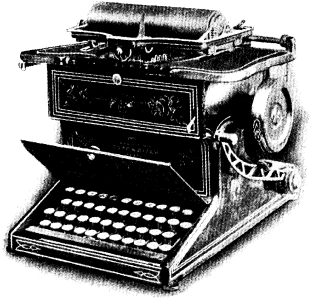
\includegraphics[width=\textwidth]{type_writer2.png}
\end{minipage}

\pause
\vfill

\textit{MRP 2019: Cross-Framework Meaning Representation Parsing}

\begin{itemize}
\item DM, PSD, EDS, UCCA and AMR parsing in English.
\item 18 teams participated.
\end{itemize}

\pause
\vfill

\textit{MRP 2020: Cross-Framework and Cross-Lingual MRP}

\begin{itemize}
\item EDS, PTG, UCCA, AMR and DRG parsing in English, Czech, German and Chinese.
\item 8 teams participated.
\end{itemize}
\end{frame}


\begin{frame}\frametitle{SemEval 2019 Task 1: Cross-lingual Semantic Parsing with UCCA}
\begin{itemize}
\item UCCA parsing in English, French and German.
\item 8 teams participated.
\item Baseline: TUPA.
\end{itemize}
\end{frame}

\begin{frame}\frametitle{SemEval 2019 Task 1}
        \begin{itemize}
            \item 
                English $\{$in-domain/out-of-domain$\} \times 
                \{$open/closed$\}$
            \item
                German in-domain $\{$open/closed$\}$
            \item
                French \textit{low-resource} (only 15 training sentences)
        \end{itemize}

\vfill
\begin{center}
  \begin{minipage}{.3\textwidth}
\includegraphics[width=\textwidth]{wikipedia.png}\end{minipage}
  \begin{minipage}{.3\textwidth}
\includegraphics[width=\textwidth]{squid.jpg}\end{minipage}
\end{center}
\end{frame}

\begin{frame}
\frametitle{SemEval 2019 Task 1}
 8 teams in total:
 \begin{itemize}
 \item
 {\it MaskParse@Deski\~{n}}  {\small Orange Labs, Aix-Marseille University}
 \item
 {\it HLT@SUDA} { \small  Soochow University}
 \item
 {\it T\"{u}Pa} {\small   University of T\"{u}bingen}
 \item
 {\it UC Davis} {\small   University of California, Davis}
 \item    
 {\it GCN-Sem}  {\small   University of Wolverhampton}
 \item
    {\it CUNY-PekingU} {\small 	 City University of New York, Peking University}
 \item
{\it DANGNT@UIT.VNU-HCM} {\small   University of Information Technology VNU-HCM}
 \item
{\it XLangMo} {\small  Zhejiang University}
\end{itemize}
\end{frame}

\begin{frame}
\frametitle{SemEval 2019 Task 1}
    \begin{figure}
        \centering
        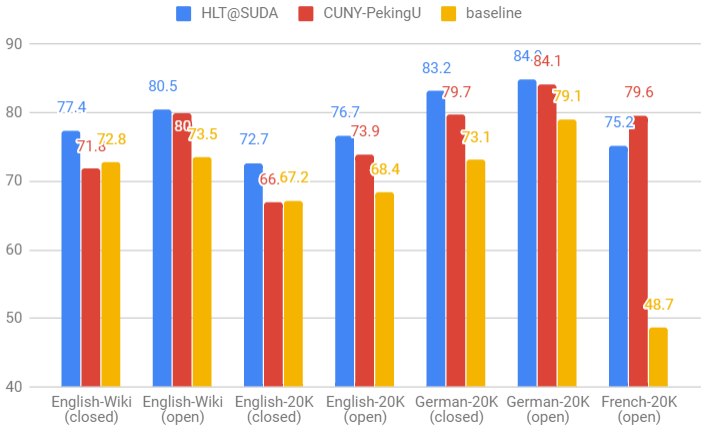
\includegraphics[width=\textwidth]{Capture}
    \end{figure}
\end{frame}

\begin{frame}
\frametitle{SemEval 2019 Task 1}

        HLT@SUDA: \\
        Neural constituency parser + multi-task + BERT \\
        French: trained on all languages, with language embedding
        
        \begin{center}
            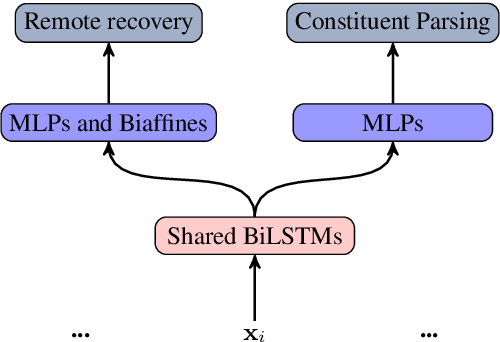
\includegraphics[width=.8\textwidth]{hltsuda3.png}
        \end{center}  
\end{frame}

\begin{frame}
\frametitle{SemEval 2019 Task 1}

        Surprisingly, results in French were close to English and German
    \begin{itemize}
        \item 
            Demonstrates viability of cross-lingual UCCA parsing
        \item
            Is this because of UCCA's stability in translation?
    \end{itemize}    
\end{frame}

\begin{frame}{MRP 2019}
\begin{itemize}
\item DM, PSD, EDS, UCCA and AMR parsing in English.
\item 18 teams participated.
\item Baseline: TUPA (generalized beyond UCCA).
\end{itemize}
\end{frame}

\pgfplotstableread{
a b c d e f shape	System	Approach	Overall	DM	PSD	EDS	UCCA	AMR
1 2 3 4 5 6 1	ERG	Composition	0.383	0.961	{}	0.952	{}	{}
1 2 3 4 5 6 3	{TUPA single}	Transition	0.577	0.555	0.518	0.810	0.276	0.447
1 2 3 4 5 6 3	{TUPA multi}	Transition	0.453	0.427	0.527	0.740	0.237	0.338
1 2 3 4 5 6 2	SJTU--NICT	Factorization	0.853	0.955	0.912	0.899	0.778	0.720
1 2 3 4 5 6 1	Saarland	Composition	0.819	0.947	0.913	0.891	0.676	0.667
1 2 3 4 5 6 3	{{\'U}FAL MRPipe}	Transition	0.747	0.849	0.763	0.675	0.732	0.718
1 2 3 4 5 6 3	{\'U}FAL--Oslo	Transition	0.344	0.805	0.609	0.306	{}	{}
1 2 3 4 5 6 2	Hitachi	Factorization	0.760	0.910	0.912	0.837	0.704	0.439
1 2 3 4 5 6 2	Amazon	Factorization	0.513	0.933	0.900	{}	{}	0.734
1 2 3 4 5 6 4	Bocharov	{}	0.065	{}	{}	{}	{}	0.327
1 2 3 4 5 6 3	HIT-SCIR	Transition	0.862	0.951	0.905	0.907	0.817	0.729
1 2 3 4 5 6 3	SJTU	Transition	0.430	0.432	0.476	0.532	0.327	0.385
1 2 3 4 5 6 2	SUDA--Alibaba	Factorization	0.840	0.923	0.856	0.918	0.784	0.717
1 2 3 4 5 6 2	JBNU	Factorization	0.465	0.940	0.879	{}	0.507	{}
1 2 3 4 5 6 4	HKUST	{}	0.245	0.370	0.353	{}	0.502	{}
1 2 3 4 5 6 2	ShanghaiTech	Factorization	0.670	0.949	0.895	0.869	{}	0.636
1 2 3 4 5 6 2	Peking	Factorization	0.711	0.944	0.894	0.945	0.772	{}
1 2 3 4 5 6 1	Peking	Composition	0.711	0.944	0.894	0.945	0.772	{}
1 2 3 4 5 6 4	Anonymous	{}	0.022	{}	0.109	{}	{}	{}
1 2 3 4 5 6 3	CUHK	Transition	0.378	0.687	0.648	0.276	0.196	0.081
}\approaches

\begin{frame}[fragile]{MRP 2019}

  \begin{center}\footnotesize
\begin{tikzpicture}
    \begin{axis}[
    enlarge x limits={abs=7mm},
    ymin=.7,ymax=1,
    clip=true,
    ymajorgrids=true,
    width=\textwidth,
    height=.9\textheight,
    xtick={1,2,3,4,5,6},
    xticklabels={Overall,DM,PSD,EDS,UCCA,AMR},
    xticklabel style={font=\small,anchor=north},
    xtick align=inside,
    xticklabel pos=left,
    tickwidth=0pt,
    axis background/.style={fill=cyan!10},
    scatter/classes={1={mark=square,red,draw opacity=.5},
                   2={mark=triangle,black,draw opacity=.5},
                   3={mark=o,blue,draw opacity=.5},
                   4={mark=x,Purple,draw opacity=0}
                  },
    scatter,only marks,mark size=7,scatter src=explicit symbolic,
    legend style={font=\tiny}
    ]
    \addplot table[x=a,y=Overall,meta=shape]{\approaches};
    \addplot table[x=b,y=DM,meta=shape]{\approaches};
    \addplot table[x=c,y=PSD,meta=shape]{\approaches};
    \addplot table[x=d,y=EDS,meta=shape]{\approaches};
    \addplot table[x=e,y=UCCA,meta=shape]{\approaches};
    \addplot table[x=f,y=AMR,meta=shape]{\approaches};
    \legend{Composition,Factorization,Transition};
    \end{axis}
\end{tikzpicture}
  \end{center}
\end{frame}

\begin{frame}
\frametitle{MRP 2019}
Winning system: HIT-SCIR \citep{Che:Dou:Xu:19}.

Transition-based parser (similar to TUPA) + efficient training + BERT.

\begin{center}
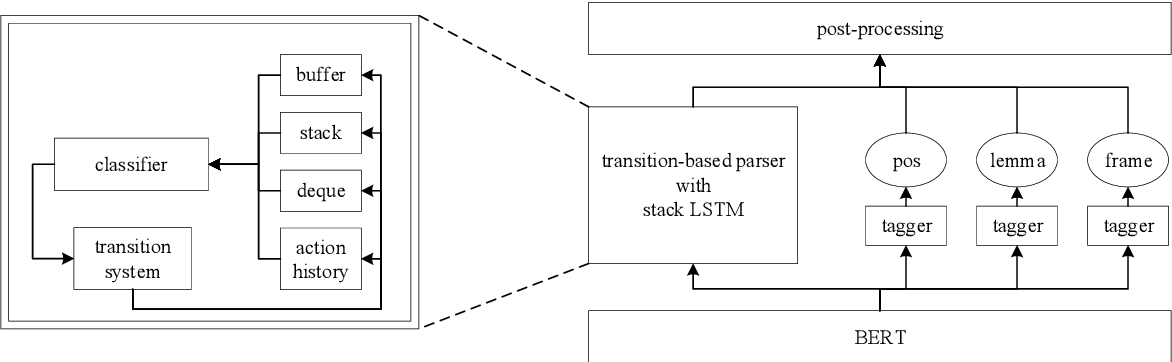
\includegraphics[width=\textwidth]{hitscir1}
\end{center}
\end{frame}

\begin{frame}{MRP 2020}
\begin{itemize}
\item EDS, PTG, UCCA, AMR and DRG parsing in English, Czech, German and Chinese.
\item 8 teams participated.
\end{itemize}
\end{frame}

\begin{frame}{MRP 2020}
\begin{center}
\begin{tabular}{lccccccccccccccc}
\toprule
 & \multicolumn{3}{c}{\textbf{EDS}} &  \multicolumn{3}{c}{\textbf{UCCA}} & \multicolumn{3}{c}{\textbf{AMR}} \\
\cmidrule(l{2pt}r{3pt}){2-4} \cmidrule(l{2pt}r{3pt}){5-7} \cmidrule(l{2pt}r{3pt}){8-10}
 & P & R & F & P & R & F & P & R & F\\
\midrule
2019 & .92 & .93 & .93 & .84 & .82 & .83 & .74 & .72 & .73 \\
2020 & .97 & .97 & .97 & .86 & .80 & .83 & .78 & .79 & .79 \\
\bottomrule
\end{tabular}
\end{center}
\end{frame}

\begin{frame}{MRP 2020}
Winning systems: \'{U}FAL \citep{Sam:Str:20} and Hitachi
    \citep{Oza:Mor:Kor:20}, encoder-decoder with pre-trained transformers.
\end{frame}

\section{Applications}

\begin{frame}
\frametitle{What can meaning representation do for NLP?}
 \begin{itemize}
 \item Incorporating linguistically informed rules
 \item Controlled evaluation by explicit criteria
 \item Inductive bias to facilitate learning
 \item Explainable models by design
 \end{itemize}
\end{frame}

\subsection{Incorporating linguistically informed rules into NLP}

\begin{frame}
\frametitle{Sentence Splitting for Text Simplification}
% https://www.aclweb.org/anthology/attachments/P18-1016.Presentation.pdf
    
    {\color{blue}Last year I read the book John authored} $\rightarrow$ \\
    \hfill {\color{red}John wrote a book.} {\color{green}I read the book.}
    
    \vfill\pause

    MT-based simplifcation is \textit{overly conservative}.
    
    \vfill\pause
    
    \textbf{Direct Semantic Splitting} before MT-based simplification
    to place each scene in its own sentence
    \citep{sulem-etal-2018-simple}.
    
    \begin{center}
        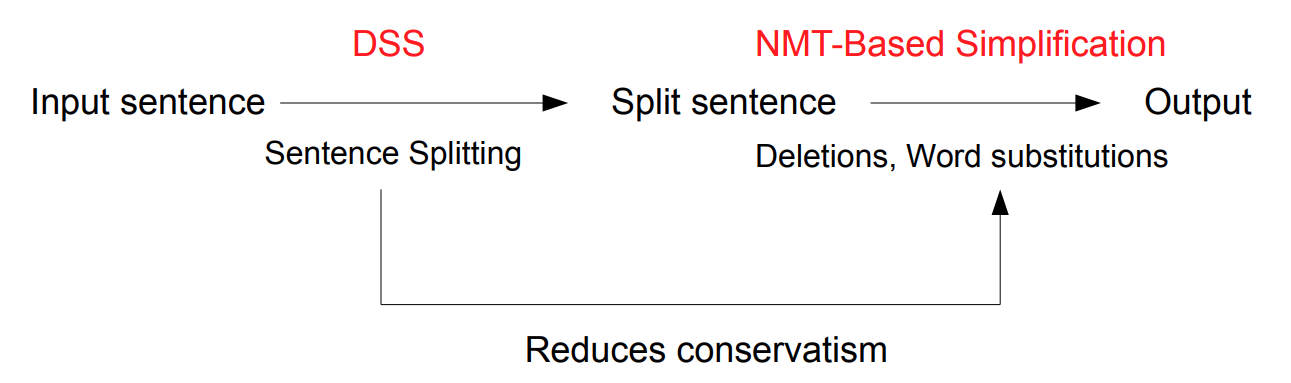
\includegraphics[width=.7\textwidth]{dss1.png}
    \end{center}
\end{frame}

\begin{frame}
\frametitle{Sentence Splitting for Text Simplification}
    \begin{center}
        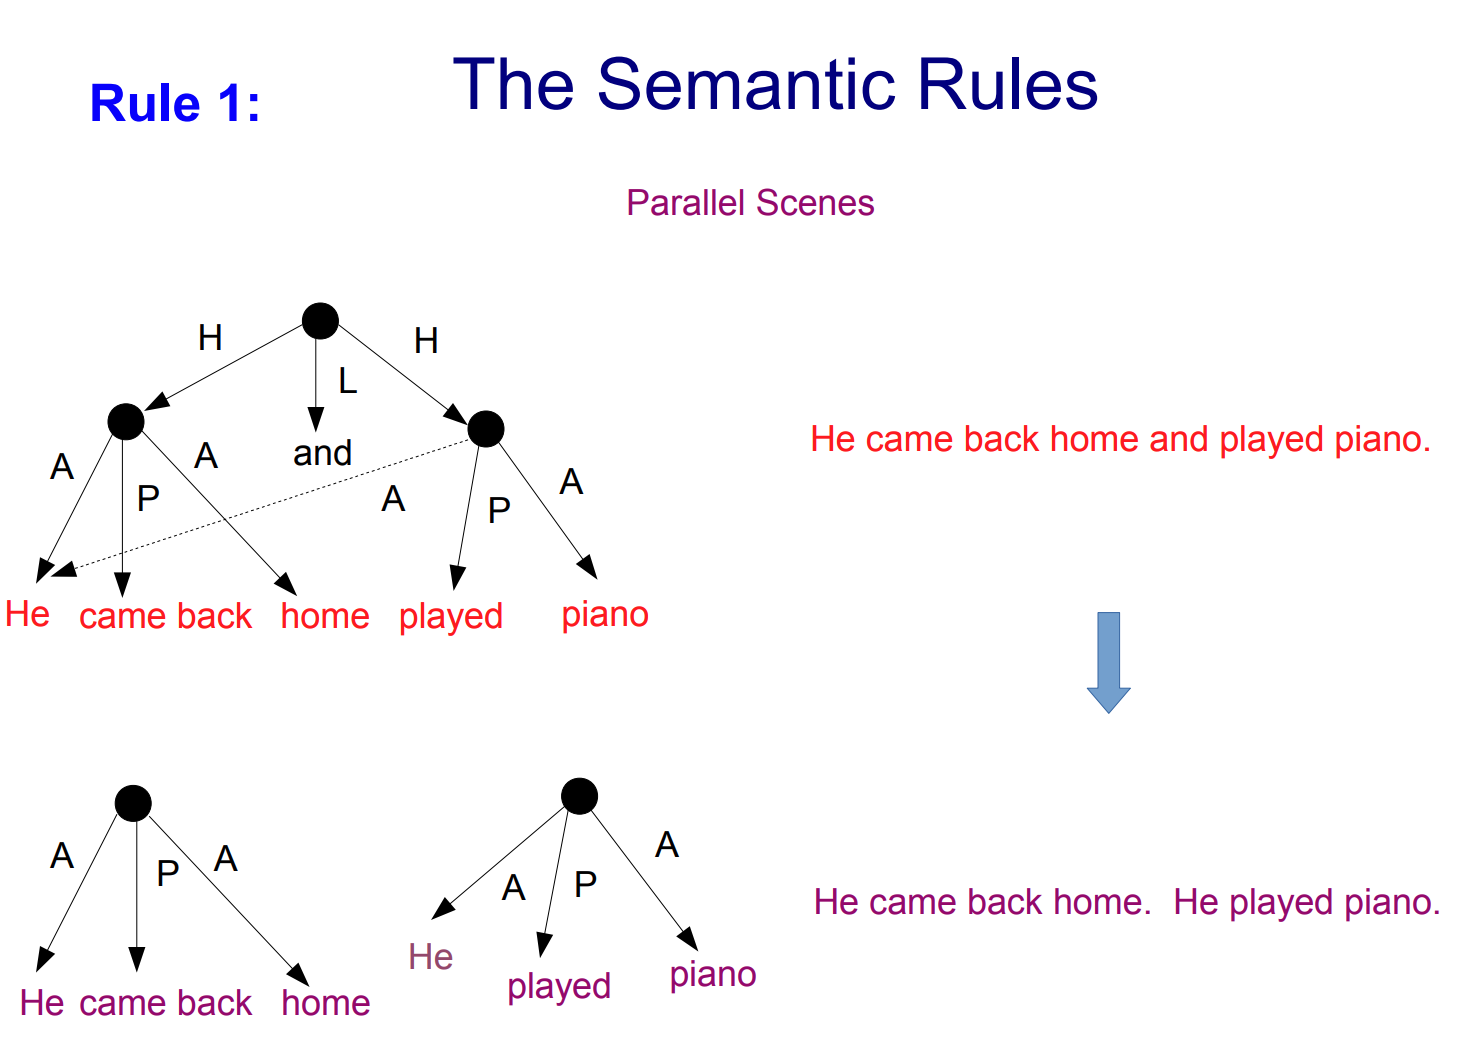
\includegraphics[width=\textwidth]{dss2.png}
    \end{center}
\end{frame}

\begin{frame}
\frametitle{Sentence Splitting for Text Simplification}
    \begin{center}
        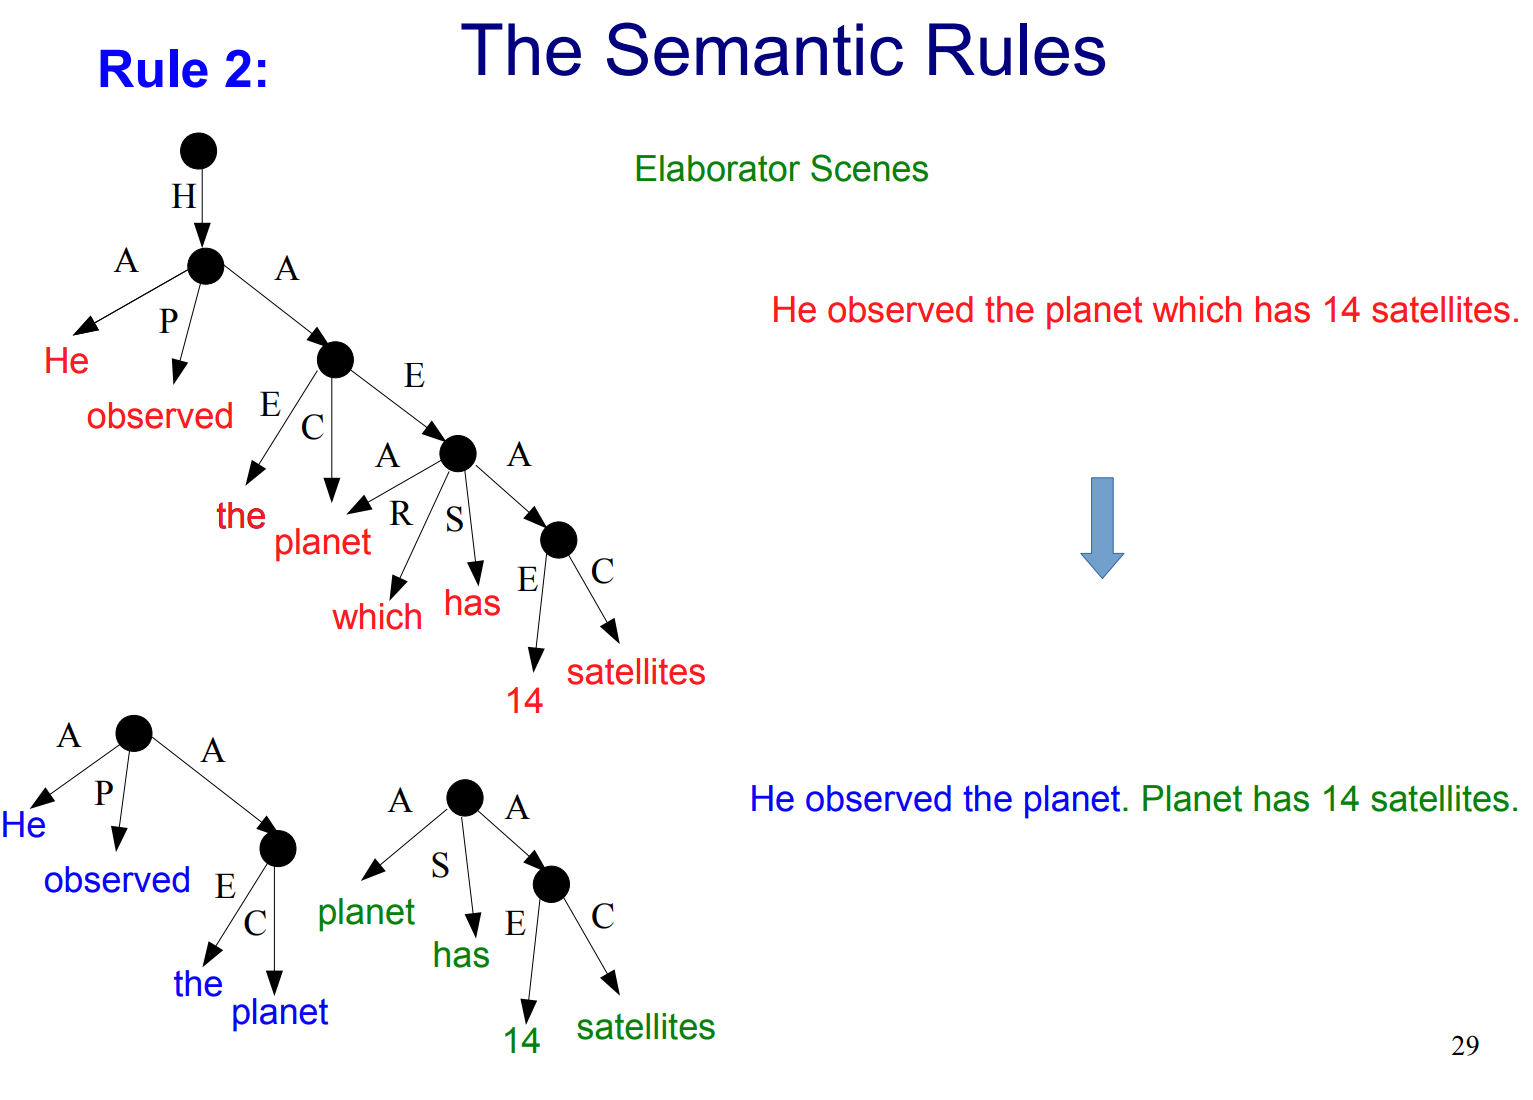
\includegraphics[width=\textwidth]{dss3.png}
    \end{center}
\end{frame}

\begin{frame}
\frametitle{Sentence Splitting for Text Simplification}
    Participant scenes are not split.
    \begin{center}
        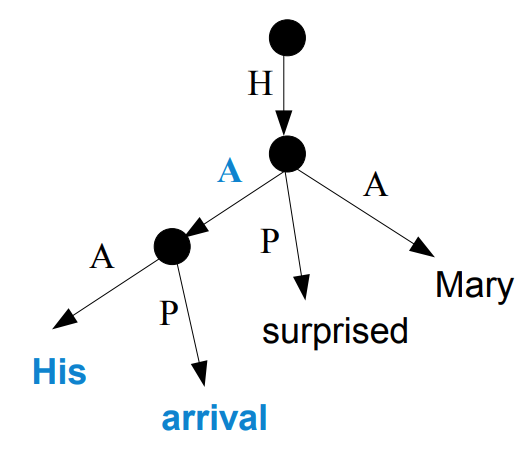
\includegraphics[width=.5\textwidth]{dss4.png}
    \end{center}
\end{frame}

\begin{frame}
\frametitle{Sentence Splitting for Text Simplification}
    {\color{blue}He observed the planet.} {\color{green}Planet has 14 satellites.}

    \vfill\pause
    
    Neural MT methods to fix grammaticality.
    \begin{center}
        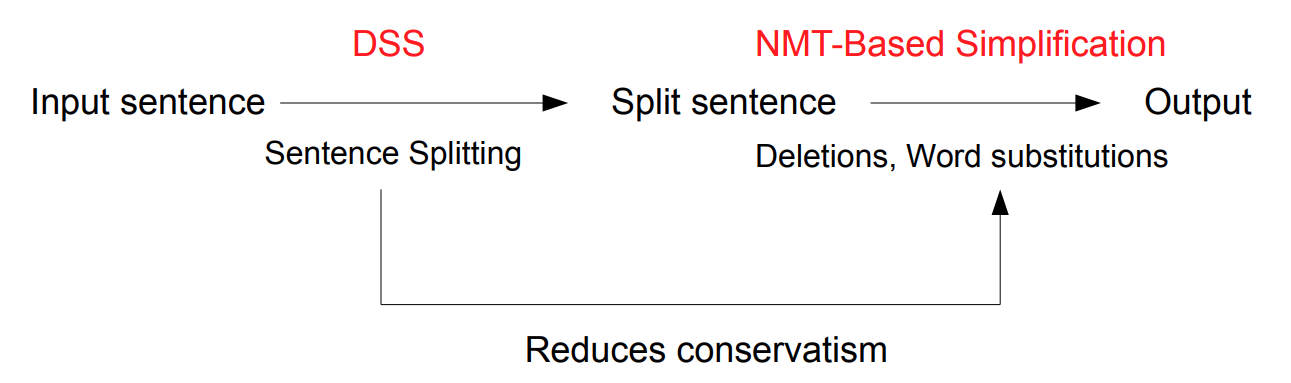
\includegraphics[width=\textwidth]{dss1.png}
    \end{center}
    
    \vfill\pause
    
    {\color{blue}He observed the planet.} {\color{green}\textbf{The planet} has 14 satellites.}
\end{frame}

% \begin{frame}
% \frametitle{Semantic Structural Decomposition for Neural Machine Translation}
%     \citep{sulem-etal-2020-semantic}.
% \end{frame}

\subsection{Controlled NLG evaluation by explicit criteria}

\begin{frame}{BLEU is Not Suitable for the Evaluation of Text Simplification}
    \textbf{BLEU}: reference-based evaluation metric for MT,
    also widely used to evaluate text simplification.
    
    \vfill\pause
    
    With sentence splitting,
    not correlated with grammaticality or meaning preservation
    \citep{sulem-etal-2018-bleu}.
    
    \vfill\pause
    
    \textit{Negatively correlated} with simplicity!
\end{frame}

\begin{frame}{Semantic Structural Evaluation for Text Simplification}
    \textbf{SAMSA}: reference-less measure of
    \textit{structural simplicity} and \textit{meaning preservation}
     \citep{sulem-etal-2018-semantic}.
     
    Same principle: \textit{one scene per sentence}.
    
    \begin{center}
        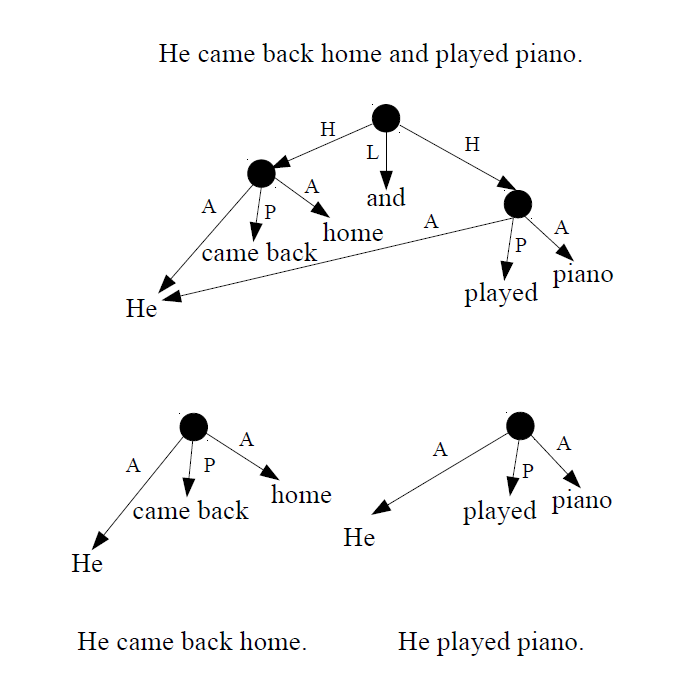
\includegraphics[width=.5\textwidth]{ucca_simplification}
    \end{center}
\end{frame}

\begin{frame}{Semantic Structural Evaluation for Text Simplification}
    \begin{center}
        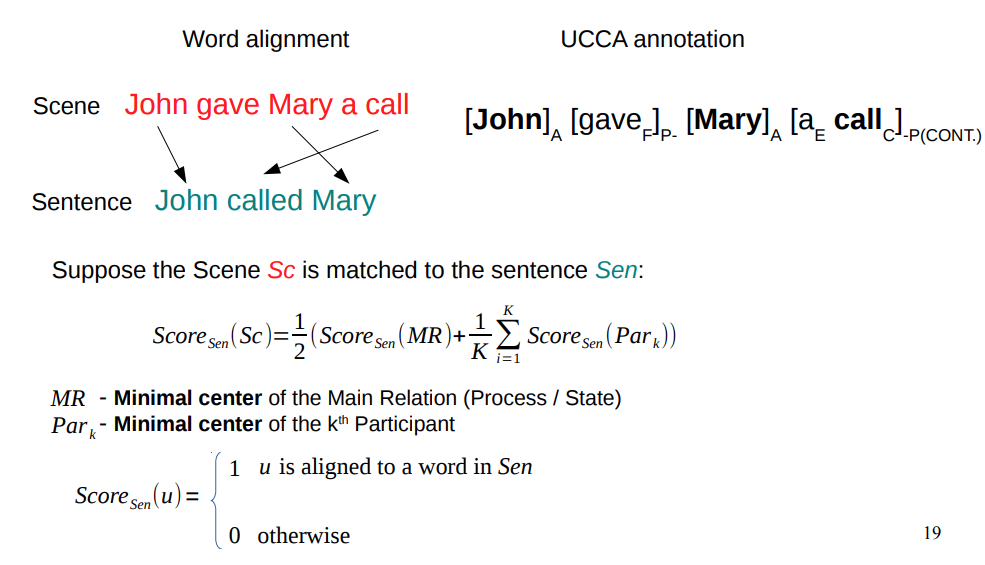
\includegraphics[width=.8\textwidth]{samsa1.png}
    \end{center}
    \begin{center}
        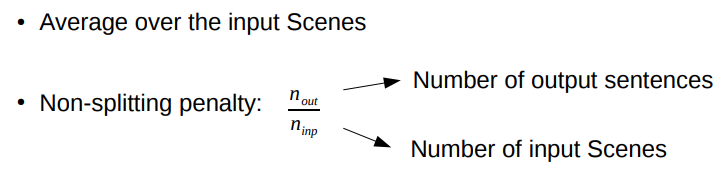
\includegraphics[width=.7\textwidth]{samsa2.png}
    \end{center}
\end{frame}

\begin{frame}{Grammatical Error Correction}
    Another text-to-text generation task.
    
    {\color{red}Ther is both sides of stories} \rightarrow \\
    \hfill {\color{blue}There are two sides to every story}
\end{frame}

\begin{frame}{Inherent Biases in Reference-based Evaluation for GEC and Text Simplification}
    Using \textit{references} for GEC evaluation underestimates performance
    \citep{choshen-abend-2018-inherent}.
    
    \begin{center}
        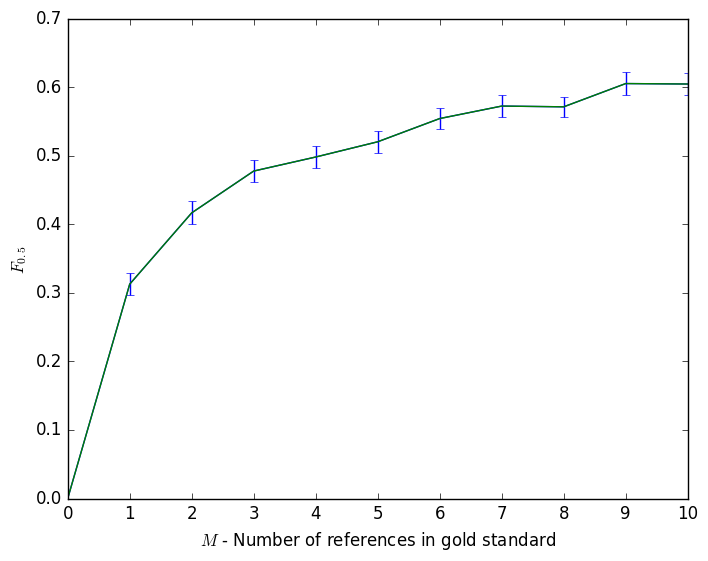
\includegraphics[width=.7\textwidth]{gec_f05.png}
    \end{center}
\end{frame}

\begin{frame}{Reference-less Measure of Faithfulness for Grammatical Error Correction}
    \begin{itemize}
        \item UCCA is \textit{applicable} to ungrammatical learner language!
        \item UCCA is \textit{stable} with respect to grammar corrections
    \end{itemize}
    
    \begin{center}
    \begin{tikzpicture}[sibling distance=3mm, level distance=7mm,
    every node/.append style={font=\rmfamily},
	every circle node/.append style={fill=black}]
    \begin{scope}[frontier/.style={distance from root=15mm},
	edge from parent path={(\tikzparentnode.center) ..
        controls +(0,-.25) and +(0,.25) .. (\tikzchildnode.north)}]
    \Tree [.\node [circle] (rootu) {};
    \edge node [auto=right]{}; \node (Heu) {He};
    \edge node[auto=right down]{}; \node (gve) {gve};
    \edge node[auto=right]{};
    [.\node [circle](an appleu) {};
    \edge node[auto=right]{}; \node (anu) {an};
    \edge node[auto=left]{}; \node (appleu) {apple};
    ]
    \edge node[auto=left]{};
    [.\node [circle](for john) {};
    \edge node[auto=right]{};\node (for) {for};
    \edge node[auto=left]{}; \node (john) {john};
    ]]
    \end{scope}
    \begin{scope}[yshift=-41mm,grow'=up,
      frontier/.style={distance from root=12mm},
      edge from parent path={(\tikzparentnode.center) ..
      controls +(0,.25) and +(0,-.25) .. (\tikzchildnode.south)}]
    \Tree [.\node [circle] (rootd) {};
    \edge node [auto=left]{}; \node (Hed) {He};
    \edge node[auto=right]{}; \node (gave) {gave};
    \edge node[auto=right]{};\node (John) {John};
    \edge node[auto=right]{};
    [.\node [circle] (an appled) {};
    \edge node[auto=left]{}; \node (and) {an};
    \edge node[auto=right]{}; \node (appled) {apple};
    ]
    ]
    \end{scope}
    \begin{scope}[dashed]
    \draw (Heu) -- (Hed);
    \draw (gve) -- (gave);
    \draw (John) -- (john);
    \draw (anu) -- (and);
    \draw (appleu) -- (appled);
    \end{scope}
    \end{tikzpicture}
    \end{center}
\end{frame}

\begin{frame}{Reference-less Measure of Faithfulness for Grammatical Error Correction}
    \textbf{USim} measures meaning preservation automatically \textit{without references}
    \citep{choshen-abend-2018-reference}.
    
    \vfill\pause
    
    Variation on standard UCCA evaluation, using unit \textit{alignment}
    between the source and target graphs.
    
    \vfill\pause
    
    Sensitive to faithfulness, not overly conservative.
    \begin{center}
        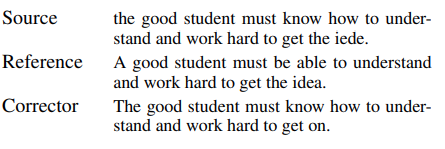
\includegraphics[width=.5\textwidth]{usim1.png}
    \end{center}
\end{frame}

% \section{Cross-linguistic Studies}

\frame{\titlepage}

\frame{
\frametitle{References}
\bibliographystyle{acl_natbib}
\tiny
\bibliography{references,anthology,mrp}
}


\end{document}
